% Capitolul 11: Foundation models pentru serii de timp
% Serii de timp -- Programele de licență Informatică economică și Cibernetică economică, Academia de Studii Economice din București
% GENERAT de latex/build_chapter11.py -- modificați generatorul, nu acest fișier.

\newcommand{\coursename}{Serii de timp}
\def\tsalang{ro}
% Preambul comun TSA -- Serii de timp / Time Series Analysis (Beamer, 16:9)
% Același design ca MFM și SFM (preluat din SFM, 5 octombrie 2026). Înainte de % Preambul comun TSA -- Serii de timp / Time Series Analysis (Beamer, 16:9)
% Același design ca MFM și SFM (preluat din SFM, 5 octombrie 2026). Înainte de % Preambul comun TSA -- Serii de timp / Time Series Analysis (Beamer, 16:9)
% Același design ca MFM și SFM (preluat din SFM, 5 octombrie 2026). Înainte de \input{../../latex/preamble} se definește
%   \newcommand{\coursename}{Time Series Analysis}      (EN)
%   \newcommand{\coursename}{Serii de timp}       (RO)  și  \def\tsalang{ro}
% Fișierele .tex se află în EN/Courses, EN/Seminars, RO/Cursuri, RO/Seminarii (două niveluri sub rădăcină).
% Deck-urile sînt generate de latex/build_chapterN.py / build_seminarN.py (vezi latex/tsa_build.py).

\documentclass[9pt, aspectratio=169, t]{beamer}
\providecommand{\coursename}{Time Series Analysis}

% Ensure content fits on slides
\setbeamersize{text margin left=8mm, text margin right=8mm}
% Smaller institute font (title page)
\setbeamerfont{institute}{size=\footnotesize}

%=============================================================================
% THEME AND STYLE CONFIGURATION
%=============================================================================
\usetheme{default}
% Using default theme for clean header/footer control

% Color Palette (matching Redispatch PDF)
\definecolor{MainBlue}{RGB}{26, 58, 110}
\definecolor{AccentBlue}{RGB}{26, 58, 110}
\definecolor{IDAred}{RGB}{205, 0, 0}
\definecolor{DarkGray}{RGB}{51, 51, 51}
\definecolor{MediumGray}{RGB}{128, 128, 128}
\definecolor{LightGray}{RGB}{248, 248, 248}
\definecolor{VeryLightGray}{RGB}{235, 235, 235}
\definecolor{KeynoteGray}{RGB}{218, 218, 218}
\definecolor{SectionGray}{RGB}{120, 120, 120}
\definecolor{FooterGray}{RGB}{100, 100, 100}
\definecolor{Crimson}{RGB}{220, 53, 69}
\definecolor{Forest}{RGB}{46, 125, 50}
\definecolor{Amber}{RGB}{181, 133, 63}
\definecolor{Orange}{RGB}{230, 126, 34}
\definecolor{Purple}{RGB}{142, 68, 173}

% Gradient background (exact Keynote 315° gradient: white to RGB 218,218,218)
\setbeamertemplate{background}{%
    \begin{tikzpicture}[remember picture, overlay]
        \shade[shading=axis, shading angle=315,
        top color=white, bottom color=KeynoteGray]
        (current page.south west) rectangle (current page.north east);
    \end{tikzpicture}%
}
% Fallback solid color for compatibility
\setbeamercolor{background canvas}{bg=}

\setbeamercolor{palette primary}{bg=MainBlue, fg=white}
\setbeamercolor{palette secondary}{bg=MainBlue!85, fg=white}
\setbeamercolor{palette tertiary}{bg=MainBlue!70, fg=white}
\setbeamercolor{structure}{fg=MainBlue}
\setbeamercolor{title}{fg=IDAred}
\setbeamercolor{frametitle}{fg=IDAred, bg=}
\setbeamercolor{block title}{bg=MainBlue, fg=white}
\setbeamercolor{block body}{bg=VeryLightGray, fg=DarkGray}
\setbeamercolor{block title alerted}{bg=Crimson, fg=white}
\setbeamercolor{block body alerted}{bg=Crimson!8, fg=DarkGray}
\setbeamercolor{block title example}{bg=Forest, fg=white}
\setbeamercolor{block body example}{bg=Forest!8, fg=DarkGray}
\setbeamercolor{item}{fg=MainBlue}

% Footer colors (override Madrid theme blue)
\setbeamercolor{author in head/foot}{fg=FooterGray, bg=}
\setbeamercolor{title in head/foot}{fg=FooterGray, bg=}
\setbeamercolor{date in head/foot}{fg=FooterGray, bg=}
\setbeamercolor{section in head/foot}{fg=FooterGray, bg=}
\setbeamercolor{subsection in head/foot}{fg=FooterGray, bg=}

% Bullet styles (apply everywhere including blocks)
\setbeamertemplate{itemize item}{\color{MainBlue}$\boxdot$}
\setbeamertemplate{itemize subitem}{\color{MainBlue}$\blacktriangleright$}
\setbeamertemplate{itemize subsubitem}{\color{MainBlue}\tiny$\bullet$}
\setbeamertemplate{itemize/enumerate body begin}{\normalsize}
\setbeamertemplate{itemize/enumerate subbody begin}{\normalsize}

% Item spacing - compact style
\setlength{\leftmargini}{10pt}       % Level 1: minimal indent
\setlength{\leftmarginii}{10pt}      % Level 2: minimal additional indent
% Compact list spacing (zero extra space before/after lists in blocks)
\makeatletter
\def\@listi{\leftmargin\leftmargini \topsep 0pt \parsep 0pt \itemsep 0pt}
\def\@listii{\leftmargin\leftmarginii \topsep 0pt \parsep 0pt \itemsep 0pt}
\makeatother

\setbeamertemplate{navigation symbols}{}

%=============================================================================
% CUSTOM HEADLINE
%=============================================================================
\setbeamertemplate{headline}{%
    \vskip10pt%
    \hbox to \paperwidth{%
        \hskip0.5cm%
        {\small\color{FooterGray}\renewcommand{\hyperlink}[2]{##2}\insertsectionhead}%
        \hfill%
        \textcolor{FooterGray}{\small\insertframenumber}%
        \hskip0.5cm%
    }%
    \vskip4pt%
    {\color{FooterGray}\hrule height 0.4pt}%
}

%=============================================================================
% CUSTOM FOOTER
%=============================================================================
\usepackage{fontawesome5}

\setbeamertemplate{footline}{%
    {\color{FooterGray}\hrule height 0.4pt}%
    \vskip4pt%
    \hbox to \paperwidth{%
        \hskip0.5cm%
        \textcolor{FooterGray}{\small\coursename}%
        \hfill%
        \raisebox{-0.1em}{%
            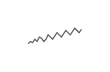
\begin{tikzpicture}[x=0.08em, y=0.08em, line width=0.4pt]
                \draw[FooterGray] (0,3) -- (1,4) -- (2,3.5) -- (3,5) -- (4,4) -- (5,6) -- (6,5.5) -- (7,4) -- (8,5) -- (9,7) -- (10,6) -- (11,5) -- (12,6.5) -- (13,8) -- (14,7) -- (15,6) -- (16,7.5) -- (17,9) -- (18,8) -- (19,7) -- (20,8.5) -- (21,10) -- (22,9) -- (23,8) -- (24,9.5);
            \end{tikzpicture}%
        }%
        \hskip0.5cm%
    }%
    \vskip6pt%
}

%=============================================================================
% PACKAGES
%=============================================================================
\usepackage[utf8]{inputenc}
\DeclareUnicodeCharacter{03B1}{\ensuremath{\alpha}}
\usepackage[T1]{fontenc}
\usepackage{amsmath, amssymb, amsthm}
\usepackage{mathtools}
\usepackage{bm}
\usepackage{tikz}
\usetikzlibrary{arrows.meta, positioning, shapes, calc, decorations.pathreplacing, shadings}
\usepackage{booktabs}
\usepackage{multirow}
\usepackage{array}
\usepackage{graphicx}
\usepackage{animate}
\usepackage{hyperref}
\usepackage{colortbl}
\usepackage{listings}
\lstset{language=Python, basicstyle=\ttfamily\scriptsize, keywordstyle=\color{MainBlue}\bfseries,
  commentstyle=\color{Forest}, stringstyle=\color{Crimson}, breaklines=true,
  frame=none, backgroundcolor=\color{VeryLightGray}, xleftmargin=2mm}
\hypersetup{colorlinks=true, linkcolor=MainBlue, urlcolor=MainBlue}
\graphicspath{{../../logos/}{../../charts/}{../../photos/}}
\usepackage{xcolor}
\hfuzz=2pt  % Suppress tiny overfull warnings (<2pt)
\vfuzz=2pt  % Suppress tiny vertical overfull warnings (<2pt)
% \mathrm in the sans-serif family of the slides (beamer resets \mathrm to the serif family at \begin{document};
% this hook runs after beamer's, so WN, Var, RMSE, ... in formulas match the surrounding text)
% Bold vectors and matrices in the same sans-serif family: \mathbf{A} in sans bold (beamer's own \mathbf came out in
% medium weight), and the bold upright Greek capitals of \boldsymbol / \bm (\bSigma, \bPhi, \boldsymbol{\Theta}) in
% cmss bold: bm.sty fixes its "boldoperators" font when it is loaded (serif cmbx), before beamer switches the
% operators to cmss, so it is reset here.
\AtBeginDocument{%
  \SetMathAlphabet{\mathrm}{normal}{\encodingdefault}{\sfdefault}{\mddefault}{n}%
  \SetMathAlphabet{\mathrm}{bold}{\encodingdefault}{\sfdefault}{bx}{n}%
  \SetMathAlphabet{\mathbf}{normal}{\encodingdefault}{\sfdefault}{bx}{n}%
  \SetMathAlphabet{\mathbf}{bold}{\encodingdefault}{\sfdefault}{bx}{n}%
  \SetSymbolFont{boldoperators}{normal}{OT1}{cmss}{bx}{n}%
  \SetSymbolFont{boldoperators}{bold}{OT1}{cmss}{bx}{n}}

%=============================================================================
% QUANTLET COMMANDS
%   \quantlet{<displayed name>}{<url>}       (generic, compatible with the older TSA decks)
%   \tsaquantlet{Ch_05}{TSA_ch5_garch}       -> https://github.com/danpele/Time-Series-Analysis/tree/main/Quantlets/Ch_05/TSA_ch5_garch
%   \qlurl{<folder>} is defined per chapter by the generator (Quantlets/Ch_NN/<folder>)
%=============================================================================
\newcommand{\tsarepo}{https://github.com/danpele/Time-Series-Analysis}
\newcommand{\tsaqlbase}{https://github.com/danpele/Time-Series-Analysis/tree/main/Quantlets}
\newcommand{\quantlet}[2]{%
    \hfill\href{#2}{%
        \raisebox{-0.15em}{
\includegraphics[height=0.7em]{ql_logo.png}}%
        \textcolor{MainBlue}{\tiny\ #1}%
    }%
}
\newcommand{\tsaquantlet}[2]{\quantlet{\detokenize{#2}}{\tsaqlbase/#1/#2}}

%=============================================================================
% NOTEBOOKS (Google Colab)
%   \colaburl{notebooks/EN/chapter5_seminar_notebook.ipynb} -> the Colab link of a file in the TSA repo
%   \nb: the chapter notebook (each seminar deck redefines it with \renewcommand)
%=============================================================================
\newcommand{\colaburl}[1]{https://colab.research.google.com/github/danpele/Time-Series-Analysis/blob/main/#1}
\newcommand{\nb}{https://colab.research.google.com/github/danpele/Time-Series-Analysis/tree/main/notebooks/EN}
\newcommand{\nbname}{notebooks/EN}

%=============================================================================
% SLIDE HELPERS (used by the generators; the same as in MFM)
%=============================================================================
% local font size for list bodies (the preamble forces \normalsize)
\newcommand{\itemsize}[1]{\setbeamertemplate{itemize/enumerate body begin}{#1}\setbeamertemplate{itemize/enumerate subbody begin}{#1}}
\newcommand{\intitle}[1]{{\hypersetup{urlcolor=white}#1}}   % white links inside coloured title bars
\newcommand{\imgcap}[1]{{\scriptsize #1}\\[0.5mm]}          % caption under a photo
\newcommand{\imgcredit}[2]{{\tiny\color{FooterGray}\href{#1}{#2}}}   % image credit: source URL, author/licence
\newcommand{\aiprompt}[1]{{\ttfamily\color{MainBlue}#1}}     % a prompt to an AI assistant

%=============================================================================
% SEMINARS: student version by default; the instructor wrapper *_solutions.tex sets \solutionstrue
%=============================================================================
\makeatletter\@ifundefined{ifsolutions}{\expandafter\newif\csname ifsolutions\endcsname}{}\makeatother
\newcommand{\solonly}[1]{\ifsolutions #1\fi}
\newcommand{\propsub}{\ifsolutions\else\framesubtitle{\ifdefined\tsalang Rezolvarea se discută la seminar\else Solution discussed in class\fi}\fi}

%=============================================================================
% APPENDIX AND CHAPTER LINKS (latex/appendix_links.py writes the calls; it also re-declares these
% macros before \begin{document}, so the decks compile with or without this preamble block)
%=============================================================================
\providecommand{\tsaapplink}[3]{\hypertarget{#2}{}\hyperlink{#1}{\beamergotobutton{#3}}}
\providecommand{\tsaappback}[2]{\begin{tikzpicture}[remember picture,overlay]\node[anchor=south east] at ([xshift=-3mm,yshift=7mm]current page.south east){\hyperlink{#1}{\beamerreturnbutton{#2}}};\end{tikzpicture}}
\providecommand{\tsachlink}[2]{\href{#1}{#2}}
\providecommand{\tsachlinkt}[2]{\href{#1}{\usebeamercolor[fg]{frametitle}#2}}

%=============================================================================
% QUANTINAR COMMAND: link către un curs Quantinar (subiecte avansate)
%=============================================================================
\newcommand{\quantinar}[2]{%
    \href{#2}{%
        \raisebox{-0.15em}{
\includegraphics[height=0.8em]{qr_logo.png}}%
        \textcolor{MainBlue}{\scriptsize\ #1}%
    }%
}

%=============================================================================
% CUSTOM TITLE PAGE
%=============================================================================
\defbeamertemplate*{title page}{hybrid}[1][]
{
    \vspace{0.2cm}
    % Logos row - top header (with clickable links)
    \begin{center}
        \href{https://www.ase.ro}{
\includegraphics[height=1.0cm]{ase_logo.png}}\hspace{0.3cm}%
        \href{https://theida.net}{
\includegraphics[height=1.0cm]{ida_logo.png}}\hspace{0.3cm}%
        \href{https://blockchain-research-center.com}{
\includegraphics[height=1.0cm]{brc_logo.png}}\hspace{0.3cm}%
        \href{https://www.ai4efin.ase.ro}{
\includegraphics[height=1.0cm]{ai4efin_logo.png}}\hspace{0.3cm}%
        \href{https://ipe.ro/new}{
\includegraphics[height=1.0cm]{acad_logo.png}}\hspace{0.3cm}%
        \href{https://www.digital-finance-msca.com}{
\includegraphics[height=1.0cm]{msca_logo.png}}%
    \end{center}

    \vspace{0.6cm}

    % Main title with Q logos on sides (with clickable links)
    \begin{center}
        \begin{minipage}{0.1\textwidth}
            \centering
            \href{https://quantlet.com}{
\includegraphics[height=1.1cm]{ql_logo.png}}
        \end{minipage}%
        \begin{minipage}{0.78\textwidth}
            \centering
            {\LARGE\bfseries\usebeamercolor[fg]{title}\inserttitle}

            \vspace{0.3cm}

            {\usebeamerfont{subtitle}\usebeamercolor[fg]{title}\insertsubtitle}
        \end{minipage}%
        \begin{minipage}{0.1\textwidth}
            \centering
            \href{https://quantinar.com}{
\includegraphics[height=1.1cm]{qr_logo.png}}
        \end{minipage}
    \end{center}

    \vspace{0.6cm}

    % Authors (left aligned)
    \hspace{0.5cm}{\usebeamerfont{author}\insertauthor}

    \vspace{0.3cm}

    % Institute/Affiliations (left aligned)
    \hspace{0.5cm}\begin{minipage}[t]{0.9\textwidth}
        \raggedright\small\insertinstitute
    \end{minipage}
}

%=============================================================================
% THEOREM ENVIRONMENTS
%=============================================================================
\theoremstyle{definition}
\setbeamertemplate{theorems}[numbered]
\ifdefined\tsalang
\newtheorem{defn}{Definiție}
\newtheorem{thm}{Teoremă}
\newtheorem{prop}{Propoziție}
\newtheorem{rmk}{Observație}
\else
\newtheorem{defn}{Definition}
\newtheorem{thm}{Theorem}
\newtheorem{prop}{Proposition}
\newtheorem{rmk}{Remark}
\fi

%=============================================================================
% CENTRED MINIPAGE (no extra vertical space)
%=============================================================================
\newenvironment{cminipage}[1]{%
    \par\noindent\hfill\begin{minipage}{#1}\ignorespaces
}{%
    \end{minipage}\hfill\null\par
}

%=============================================================================
% CUSTOM COMMANDS
%=============================================================================
\newcommand{\E}{\mathbb{E}}
\newcommand{\Var}{\text{Var}}
\newcommand{\Cov}{\text{Cov}}
\newcommand{\Corr}{\text{Corr}}
\newcommand{\R}{\mathbb{R}}
\newcommand{\N}{\mathbb{N}}
\newcommand{\Z}{\mathbb{Z}}
\newcommand{\B}{\mathbf{B}}
\newcommand{\imark}{\textcolor{MainBlue}{\textbullet}}
\newcommand{\RMSE}{\text{RMSE}}
\newcommand{\MAE}{\text{MAE}}
\newcommand{\MAPE}{\text{MAPE}}

% Boldface vector/matrix commands (VAR, VECM, state space; also used by the older TSA decks)
\newcommand{\bY}{\mathbf{Y}}
\newcommand{\bX}{\mathbf{X}}
\newcommand{\bA}{\mathbf{A}}
\newcommand{\bB}{\mathbf{B}}
\newcommand{\bepsilon}{\boldsymbol{\varepsilon}}
\newcommand{\bSigma}{\boldsymbol{\Sigma}}
\newcommand{\bPhi}{\boldsymbol{\Phi}}
\newcommand{\bGamma}{\boldsymbol{\Gamma}}
\newcommand{\bPi}{\boldsymbol{\Pi}}
\newcommand{\bc}{\mathbf{c}}
\newcommand{\balpha}{\boldsymbol{\alpha}}
\newcommand{\bbeta}{\boldsymbol{\beta}}
\newcommand{\bvarepsilon}{\boldsymbol{\varepsilon}}

% Legacy seminar marks (older TSA seminar decks)
\newcommand{\correct}{\textcolor{Forest}{\checkmark}}
\newcommand{\incorrect}{\textcolor{Crimson}{\texttimes}}
 se definește
%   \newcommand{\coursename}{Time Series Analysis}      (EN)
%   \newcommand{\coursename}{Serii de timp}       (RO)  și  \def\tsalang{ro}
% Fișierele .tex se află în EN/Courses, EN/Seminars, RO/Cursuri, RO/Seminarii (două niveluri sub rădăcină).
% Deck-urile sînt generate de latex/build_chapterN.py / build_seminarN.py (vezi latex/tsa_build.py).

\documentclass[9pt, aspectratio=169, t]{beamer}
\providecommand{\coursename}{Time Series Analysis}

% Ensure content fits on slides
\setbeamersize{text margin left=8mm, text margin right=8mm}
% Smaller institute font (title page)
\setbeamerfont{institute}{size=\footnotesize}

%=============================================================================
% THEME AND STYLE CONFIGURATION
%=============================================================================
\usetheme{default}
% Using default theme for clean header/footer control

% Color Palette (matching Redispatch PDF)
\definecolor{MainBlue}{RGB}{26, 58, 110}
\definecolor{AccentBlue}{RGB}{26, 58, 110}
\definecolor{IDAred}{RGB}{205, 0, 0}
\definecolor{DarkGray}{RGB}{51, 51, 51}
\definecolor{MediumGray}{RGB}{128, 128, 128}
\definecolor{LightGray}{RGB}{248, 248, 248}
\definecolor{VeryLightGray}{RGB}{235, 235, 235}
\definecolor{KeynoteGray}{RGB}{218, 218, 218}
\definecolor{SectionGray}{RGB}{120, 120, 120}
\definecolor{FooterGray}{RGB}{100, 100, 100}
\definecolor{Crimson}{RGB}{220, 53, 69}
\definecolor{Forest}{RGB}{46, 125, 50}
\definecolor{Amber}{RGB}{181, 133, 63}
\definecolor{Orange}{RGB}{230, 126, 34}
\definecolor{Purple}{RGB}{142, 68, 173}

% Gradient background (exact Keynote 315° gradient: white to RGB 218,218,218)
\setbeamertemplate{background}{%
    \begin{tikzpicture}[remember picture, overlay]
        \shade[shading=axis, shading angle=315,
        top color=white, bottom color=KeynoteGray]
        (current page.south west) rectangle (current page.north east);
    \end{tikzpicture}%
}
% Fallback solid color for compatibility
\setbeamercolor{background canvas}{bg=}

\setbeamercolor{palette primary}{bg=MainBlue, fg=white}
\setbeamercolor{palette secondary}{bg=MainBlue!85, fg=white}
\setbeamercolor{palette tertiary}{bg=MainBlue!70, fg=white}
\setbeamercolor{structure}{fg=MainBlue}
\setbeamercolor{title}{fg=IDAred}
\setbeamercolor{frametitle}{fg=IDAred, bg=}
\setbeamercolor{block title}{bg=MainBlue, fg=white}
\setbeamercolor{block body}{bg=VeryLightGray, fg=DarkGray}
\setbeamercolor{block title alerted}{bg=Crimson, fg=white}
\setbeamercolor{block body alerted}{bg=Crimson!8, fg=DarkGray}
\setbeamercolor{block title example}{bg=Forest, fg=white}
\setbeamercolor{block body example}{bg=Forest!8, fg=DarkGray}
\setbeamercolor{item}{fg=MainBlue}

% Footer colors (override Madrid theme blue)
\setbeamercolor{author in head/foot}{fg=FooterGray, bg=}
\setbeamercolor{title in head/foot}{fg=FooterGray, bg=}
\setbeamercolor{date in head/foot}{fg=FooterGray, bg=}
\setbeamercolor{section in head/foot}{fg=FooterGray, bg=}
\setbeamercolor{subsection in head/foot}{fg=FooterGray, bg=}

% Bullet styles (apply everywhere including blocks)
\setbeamertemplate{itemize item}{\color{MainBlue}$\boxdot$}
\setbeamertemplate{itemize subitem}{\color{MainBlue}$\blacktriangleright$}
\setbeamertemplate{itemize subsubitem}{\color{MainBlue}\tiny$\bullet$}
\setbeamertemplate{itemize/enumerate body begin}{\normalsize}
\setbeamertemplate{itemize/enumerate subbody begin}{\normalsize}

% Item spacing - compact style
\setlength{\leftmargini}{10pt}       % Level 1: minimal indent
\setlength{\leftmarginii}{10pt}      % Level 2: minimal additional indent
% Compact list spacing (zero extra space before/after lists in blocks)
\makeatletter
\def\@listi{\leftmargin\leftmargini \topsep 0pt \parsep 0pt \itemsep 0pt}
\def\@listii{\leftmargin\leftmarginii \topsep 0pt \parsep 0pt \itemsep 0pt}
\makeatother

\setbeamertemplate{navigation symbols}{}

%=============================================================================
% CUSTOM HEADLINE
%=============================================================================
\setbeamertemplate{headline}{%
    \vskip10pt%
    \hbox to \paperwidth{%
        \hskip0.5cm%
        {\small\color{FooterGray}\renewcommand{\hyperlink}[2]{##2}\insertsectionhead}%
        \hfill%
        \textcolor{FooterGray}{\small\insertframenumber}%
        \hskip0.5cm%
    }%
    \vskip4pt%
    {\color{FooterGray}\hrule height 0.4pt}%
}

%=============================================================================
% CUSTOM FOOTER
%=============================================================================
\usepackage{fontawesome5}

\setbeamertemplate{footline}{%
    {\color{FooterGray}\hrule height 0.4pt}%
    \vskip4pt%
    \hbox to \paperwidth{%
        \hskip0.5cm%
        \textcolor{FooterGray}{\small\coursename}%
        \hfill%
        \raisebox{-0.1em}{%
            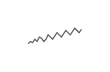
\begin{tikzpicture}[x=0.08em, y=0.08em, line width=0.4pt]
                \draw[FooterGray] (0,3) -- (1,4) -- (2,3.5) -- (3,5) -- (4,4) -- (5,6) -- (6,5.5) -- (7,4) -- (8,5) -- (9,7) -- (10,6) -- (11,5) -- (12,6.5) -- (13,8) -- (14,7) -- (15,6) -- (16,7.5) -- (17,9) -- (18,8) -- (19,7) -- (20,8.5) -- (21,10) -- (22,9) -- (23,8) -- (24,9.5);
            \end{tikzpicture}%
        }%
        \hskip0.5cm%
    }%
    \vskip6pt%
}

%=============================================================================
% PACKAGES
%=============================================================================
\usepackage[utf8]{inputenc}
\DeclareUnicodeCharacter{03B1}{\ensuremath{\alpha}}
\usepackage[T1]{fontenc}
\usepackage{amsmath, amssymb, amsthm}
\usepackage{mathtools}
\usepackage{bm}
\usepackage{tikz}
\usetikzlibrary{arrows.meta, positioning, shapes, calc, decorations.pathreplacing, shadings}
\usepackage{booktabs}
\usepackage{multirow}
\usepackage{array}
\usepackage{graphicx}
\usepackage{animate}
\usepackage{hyperref}
\usepackage{colortbl}
\usepackage{listings}
\lstset{language=Python, basicstyle=\ttfamily\scriptsize, keywordstyle=\color{MainBlue}\bfseries,
  commentstyle=\color{Forest}, stringstyle=\color{Crimson}, breaklines=true,
  frame=none, backgroundcolor=\color{VeryLightGray}, xleftmargin=2mm}
\hypersetup{colorlinks=true, linkcolor=MainBlue, urlcolor=MainBlue}
\graphicspath{{../../logos/}{../../charts/}{../../photos/}}
\usepackage{xcolor}
\hfuzz=2pt  % Suppress tiny overfull warnings (<2pt)
\vfuzz=2pt  % Suppress tiny vertical overfull warnings (<2pt)
% \mathrm in the sans-serif family of the slides (beamer resets \mathrm to the serif family at \begin{document};
% this hook runs after beamer's, so WN, Var, RMSE, ... in formulas match the surrounding text)
% Bold vectors and matrices in the same sans-serif family: \mathbf{A} in sans bold (beamer's own \mathbf came out in
% medium weight), and the bold upright Greek capitals of \boldsymbol / \bm (\bSigma, \bPhi, \boldsymbol{\Theta}) in
% cmss bold: bm.sty fixes its "boldoperators" font when it is loaded (serif cmbx), before beamer switches the
% operators to cmss, so it is reset here.
\AtBeginDocument{%
  \SetMathAlphabet{\mathrm}{normal}{\encodingdefault}{\sfdefault}{\mddefault}{n}%
  \SetMathAlphabet{\mathrm}{bold}{\encodingdefault}{\sfdefault}{bx}{n}%
  \SetMathAlphabet{\mathbf}{normal}{\encodingdefault}{\sfdefault}{bx}{n}%
  \SetMathAlphabet{\mathbf}{bold}{\encodingdefault}{\sfdefault}{bx}{n}%
  \SetSymbolFont{boldoperators}{normal}{OT1}{cmss}{bx}{n}%
  \SetSymbolFont{boldoperators}{bold}{OT1}{cmss}{bx}{n}}

%=============================================================================
% QUANTLET COMMANDS
%   \quantlet{<displayed name>}{<url>}       (generic, compatible with the older TSA decks)
%   \tsaquantlet{Ch_05}{TSA_ch5_garch}       -> https://github.com/danpele/Time-Series-Analysis/tree/main/Quantlets/Ch_05/TSA_ch5_garch
%   \qlurl{<folder>} is defined per chapter by the generator (Quantlets/Ch_NN/<folder>)
%=============================================================================
\newcommand{\tsarepo}{https://github.com/danpele/Time-Series-Analysis}
\newcommand{\tsaqlbase}{https://github.com/danpele/Time-Series-Analysis/tree/main/Quantlets}
\newcommand{\quantlet}[2]{%
    \hfill\href{#2}{%
        \raisebox{-0.15em}{
\includegraphics[height=0.7em]{ql_logo.png}}%
        \textcolor{MainBlue}{\tiny\ #1}%
    }%
}
\newcommand{\tsaquantlet}[2]{\quantlet{\detokenize{#2}}{\tsaqlbase/#1/#2}}

%=============================================================================
% NOTEBOOKS (Google Colab)
%   \colaburl{notebooks/EN/chapter5_seminar_notebook.ipynb} -> the Colab link of a file in the TSA repo
%   \nb: the chapter notebook (each seminar deck redefines it with \renewcommand)
%=============================================================================
\newcommand{\colaburl}[1]{https://colab.research.google.com/github/danpele/Time-Series-Analysis/blob/main/#1}
\newcommand{\nb}{https://colab.research.google.com/github/danpele/Time-Series-Analysis/tree/main/notebooks/EN}
\newcommand{\nbname}{notebooks/EN}

%=============================================================================
% SLIDE HELPERS (used by the generators; the same as in MFM)
%=============================================================================
% local font size for list bodies (the preamble forces \normalsize)
\newcommand{\itemsize}[1]{\setbeamertemplate{itemize/enumerate body begin}{#1}\setbeamertemplate{itemize/enumerate subbody begin}{#1}}
\newcommand{\intitle}[1]{{\hypersetup{urlcolor=white}#1}}   % white links inside coloured title bars
\newcommand{\imgcap}[1]{{\scriptsize #1}\\[0.5mm]}          % caption under a photo
\newcommand{\imgcredit}[2]{{\tiny\color{FooterGray}\href{#1}{#2}}}   % image credit: source URL, author/licence
\newcommand{\aiprompt}[1]{{\ttfamily\color{MainBlue}#1}}     % a prompt to an AI assistant

%=============================================================================
% SEMINARS: student version by default; the instructor wrapper *_solutions.tex sets \solutionstrue
%=============================================================================
\makeatletter\@ifundefined{ifsolutions}{\expandafter\newif\csname ifsolutions\endcsname}{}\makeatother
\newcommand{\solonly}[1]{\ifsolutions #1\fi}
\newcommand{\propsub}{\ifsolutions\else\framesubtitle{\ifdefined\tsalang Rezolvarea se discută la seminar\else Solution discussed in class\fi}\fi}

%=============================================================================
% APPENDIX AND CHAPTER LINKS (latex/appendix_links.py writes the calls; it also re-declares these
% macros before \begin{document}, so the decks compile with or without this preamble block)
%=============================================================================
\providecommand{\tsaapplink}[3]{\hypertarget{#2}{}\hyperlink{#1}{\beamergotobutton{#3}}}
\providecommand{\tsaappback}[2]{\begin{tikzpicture}[remember picture,overlay]\node[anchor=south east] at ([xshift=-3mm,yshift=7mm]current page.south east){\hyperlink{#1}{\beamerreturnbutton{#2}}};\end{tikzpicture}}
\providecommand{\tsachlink}[2]{\href{#1}{#2}}
\providecommand{\tsachlinkt}[2]{\href{#1}{\usebeamercolor[fg]{frametitle}#2}}

%=============================================================================
% QUANTINAR COMMAND: link către un curs Quantinar (subiecte avansate)
%=============================================================================
\newcommand{\quantinar}[2]{%
    \href{#2}{%
        \raisebox{-0.15em}{
\includegraphics[height=0.8em]{qr_logo.png}}%
        \textcolor{MainBlue}{\scriptsize\ #1}%
    }%
}

%=============================================================================
% CUSTOM TITLE PAGE
%=============================================================================
\defbeamertemplate*{title page}{hybrid}[1][]
{
    \vspace{0.2cm}
    % Logos row - top header (with clickable links)
    \begin{center}
        \href{https://www.ase.ro}{
\includegraphics[height=1.0cm]{ase_logo.png}}\hspace{0.3cm}%
        \href{https://theida.net}{
\includegraphics[height=1.0cm]{ida_logo.png}}\hspace{0.3cm}%
        \href{https://blockchain-research-center.com}{
\includegraphics[height=1.0cm]{brc_logo.png}}\hspace{0.3cm}%
        \href{https://www.ai4efin.ase.ro}{
\includegraphics[height=1.0cm]{ai4efin_logo.png}}\hspace{0.3cm}%
        \href{https://ipe.ro/new}{
\includegraphics[height=1.0cm]{acad_logo.png}}\hspace{0.3cm}%
        \href{https://www.digital-finance-msca.com}{
\includegraphics[height=1.0cm]{msca_logo.png}}%
    \end{center}

    \vspace{0.6cm}

    % Main title with Q logos on sides (with clickable links)
    \begin{center}
        \begin{minipage}{0.1\textwidth}
            \centering
            \href{https://quantlet.com}{
\includegraphics[height=1.1cm]{ql_logo.png}}
        \end{minipage}%
        \begin{minipage}{0.78\textwidth}
            \centering
            {\LARGE\bfseries\usebeamercolor[fg]{title}\inserttitle}

            \vspace{0.3cm}

            {\usebeamerfont{subtitle}\usebeamercolor[fg]{title}\insertsubtitle}
        \end{minipage}%
        \begin{minipage}{0.1\textwidth}
            \centering
            \href{https://quantinar.com}{
\includegraphics[height=1.1cm]{qr_logo.png}}
        \end{minipage}
    \end{center}

    \vspace{0.6cm}

    % Authors (left aligned)
    \hspace{0.5cm}{\usebeamerfont{author}\insertauthor}

    \vspace{0.3cm}

    % Institute/Affiliations (left aligned)
    \hspace{0.5cm}\begin{minipage}[t]{0.9\textwidth}
        \raggedright\small\insertinstitute
    \end{minipage}
}

%=============================================================================
% THEOREM ENVIRONMENTS
%=============================================================================
\theoremstyle{definition}
\setbeamertemplate{theorems}[numbered]
\ifdefined\tsalang
\newtheorem{defn}{Definiție}
\newtheorem{thm}{Teoremă}
\newtheorem{prop}{Propoziție}
\newtheorem{rmk}{Observație}
\else
\newtheorem{defn}{Definition}
\newtheorem{thm}{Theorem}
\newtheorem{prop}{Proposition}
\newtheorem{rmk}{Remark}
\fi

%=============================================================================
% CENTRED MINIPAGE (no extra vertical space)
%=============================================================================
\newenvironment{cminipage}[1]{%
    \par\noindent\hfill\begin{minipage}{#1}\ignorespaces
}{%
    \end{minipage}\hfill\null\par
}

%=============================================================================
% CUSTOM COMMANDS
%=============================================================================
\newcommand{\E}{\mathbb{E}}
\newcommand{\Var}{\text{Var}}
\newcommand{\Cov}{\text{Cov}}
\newcommand{\Corr}{\text{Corr}}
\newcommand{\R}{\mathbb{R}}
\newcommand{\N}{\mathbb{N}}
\newcommand{\Z}{\mathbb{Z}}
\newcommand{\B}{\mathbf{B}}
\newcommand{\imark}{\textcolor{MainBlue}{\textbullet}}
\newcommand{\RMSE}{\text{RMSE}}
\newcommand{\MAE}{\text{MAE}}
\newcommand{\MAPE}{\text{MAPE}}

% Boldface vector/matrix commands (VAR, VECM, state space; also used by the older TSA decks)
\newcommand{\bY}{\mathbf{Y}}
\newcommand{\bX}{\mathbf{X}}
\newcommand{\bA}{\mathbf{A}}
\newcommand{\bB}{\mathbf{B}}
\newcommand{\bepsilon}{\boldsymbol{\varepsilon}}
\newcommand{\bSigma}{\boldsymbol{\Sigma}}
\newcommand{\bPhi}{\boldsymbol{\Phi}}
\newcommand{\bGamma}{\boldsymbol{\Gamma}}
\newcommand{\bPi}{\boldsymbol{\Pi}}
\newcommand{\bc}{\mathbf{c}}
\newcommand{\balpha}{\boldsymbol{\alpha}}
\newcommand{\bbeta}{\boldsymbol{\beta}}
\newcommand{\bvarepsilon}{\boldsymbol{\varepsilon}}

% Legacy seminar marks (older TSA seminar decks)
\newcommand{\correct}{\textcolor{Forest}{\checkmark}}
\newcommand{\incorrect}{\textcolor{Crimson}{\texttimes}}
 se definește
%   \newcommand{\coursename}{Time Series Analysis}      (EN)
%   \newcommand{\coursename}{Serii de timp}       (RO)  și  \def\tsalang{ro}
% Fișierele .tex se află în EN/Courses, EN/Seminars, RO/Cursuri, RO/Seminarii (două niveluri sub rădăcină).
% Deck-urile sînt generate de latex/build_chapterN.py / build_seminarN.py (vezi latex/tsa_build.py).

\documentclass[9pt, aspectratio=169, t]{beamer}
\providecommand{\coursename}{Time Series Analysis}

% Ensure content fits on slides
\setbeamersize{text margin left=8mm, text margin right=8mm}
% Smaller institute font (title page)
\setbeamerfont{institute}{size=\footnotesize}

%=============================================================================
% THEME AND STYLE CONFIGURATION
%=============================================================================
\usetheme{default}
% Using default theme for clean header/footer control

% Color Palette (matching Redispatch PDF)
\definecolor{MainBlue}{RGB}{26, 58, 110}
\definecolor{AccentBlue}{RGB}{26, 58, 110}
\definecolor{IDAred}{RGB}{205, 0, 0}
\definecolor{DarkGray}{RGB}{51, 51, 51}
\definecolor{MediumGray}{RGB}{128, 128, 128}
\definecolor{LightGray}{RGB}{248, 248, 248}
\definecolor{VeryLightGray}{RGB}{235, 235, 235}
\definecolor{KeynoteGray}{RGB}{218, 218, 218}
\definecolor{SectionGray}{RGB}{120, 120, 120}
\definecolor{FooterGray}{RGB}{100, 100, 100}
\definecolor{Crimson}{RGB}{220, 53, 69}
\definecolor{Forest}{RGB}{46, 125, 50}
\definecolor{Amber}{RGB}{181, 133, 63}
\definecolor{Orange}{RGB}{230, 126, 34}
\definecolor{Purple}{RGB}{142, 68, 173}

% Gradient background (exact Keynote 315° gradient: white to RGB 218,218,218)
\setbeamertemplate{background}{%
    \begin{tikzpicture}[remember picture, overlay]
        \shade[shading=axis, shading angle=315,
        top color=white, bottom color=KeynoteGray]
        (current page.south west) rectangle (current page.north east);
    \end{tikzpicture}%
}
% Fallback solid color for compatibility
\setbeamercolor{background canvas}{bg=}

\setbeamercolor{palette primary}{bg=MainBlue, fg=white}
\setbeamercolor{palette secondary}{bg=MainBlue!85, fg=white}
\setbeamercolor{palette tertiary}{bg=MainBlue!70, fg=white}
\setbeamercolor{structure}{fg=MainBlue}
\setbeamercolor{title}{fg=IDAred}
\setbeamercolor{frametitle}{fg=IDAred, bg=}
\setbeamercolor{block title}{bg=MainBlue, fg=white}
\setbeamercolor{block body}{bg=VeryLightGray, fg=DarkGray}
\setbeamercolor{block title alerted}{bg=Crimson, fg=white}
\setbeamercolor{block body alerted}{bg=Crimson!8, fg=DarkGray}
\setbeamercolor{block title example}{bg=Forest, fg=white}
\setbeamercolor{block body example}{bg=Forest!8, fg=DarkGray}
\setbeamercolor{item}{fg=MainBlue}

% Footer colors (override Madrid theme blue)
\setbeamercolor{author in head/foot}{fg=FooterGray, bg=}
\setbeamercolor{title in head/foot}{fg=FooterGray, bg=}
\setbeamercolor{date in head/foot}{fg=FooterGray, bg=}
\setbeamercolor{section in head/foot}{fg=FooterGray, bg=}
\setbeamercolor{subsection in head/foot}{fg=FooterGray, bg=}

% Bullet styles (apply everywhere including blocks)
\setbeamertemplate{itemize item}{\color{MainBlue}$\boxdot$}
\setbeamertemplate{itemize subitem}{\color{MainBlue}$\blacktriangleright$}
\setbeamertemplate{itemize subsubitem}{\color{MainBlue}\tiny$\bullet$}
\setbeamertemplate{itemize/enumerate body begin}{\normalsize}
\setbeamertemplate{itemize/enumerate subbody begin}{\normalsize}

% Item spacing - compact style
\setlength{\leftmargini}{10pt}       % Level 1: minimal indent
\setlength{\leftmarginii}{10pt}      % Level 2: minimal additional indent
% Compact list spacing (zero extra space before/after lists in blocks)
\makeatletter
\def\@listi{\leftmargin\leftmargini \topsep 0pt \parsep 0pt \itemsep 0pt}
\def\@listii{\leftmargin\leftmarginii \topsep 0pt \parsep 0pt \itemsep 0pt}
\makeatother

\setbeamertemplate{navigation symbols}{}

%=============================================================================
% CUSTOM HEADLINE
%=============================================================================
\setbeamertemplate{headline}{%
    \vskip10pt%
    \hbox to \paperwidth{%
        \hskip0.5cm%
        {\small\color{FooterGray}\renewcommand{\hyperlink}[2]{##2}\insertsectionhead}%
        \hfill%
        \textcolor{FooterGray}{\small\insertframenumber}%
        \hskip0.5cm%
    }%
    \vskip4pt%
    {\color{FooterGray}\hrule height 0.4pt}%
}

%=============================================================================
% CUSTOM FOOTER
%=============================================================================
\usepackage{fontawesome5}

\setbeamertemplate{footline}{%
    {\color{FooterGray}\hrule height 0.4pt}%
    \vskip4pt%
    \hbox to \paperwidth{%
        \hskip0.5cm%
        \textcolor{FooterGray}{\small\coursename}%
        \hfill%
        \raisebox{-0.1em}{%
            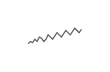
\begin{tikzpicture}[x=0.08em, y=0.08em, line width=0.4pt]
                \draw[FooterGray] (0,3) -- (1,4) -- (2,3.5) -- (3,5) -- (4,4) -- (5,6) -- (6,5.5) -- (7,4) -- (8,5) -- (9,7) -- (10,6) -- (11,5) -- (12,6.5) -- (13,8) -- (14,7) -- (15,6) -- (16,7.5) -- (17,9) -- (18,8) -- (19,7) -- (20,8.5) -- (21,10) -- (22,9) -- (23,8) -- (24,9.5);
            \end{tikzpicture}%
        }%
        \hskip0.5cm%
    }%
    \vskip6pt%
}

%=============================================================================
% PACKAGES
%=============================================================================
\usepackage[utf8]{inputenc}
\DeclareUnicodeCharacter{03B1}{\ensuremath{\alpha}}
\usepackage[T1]{fontenc}
\usepackage{amsmath, amssymb, amsthm}
\usepackage{mathtools}
\usepackage{bm}
\usepackage{tikz}
\usetikzlibrary{arrows.meta, positioning, shapes, calc, decorations.pathreplacing, shadings}
\usepackage{booktabs}
\usepackage{multirow}
\usepackage{array}
\usepackage{graphicx}
\usepackage{animate}
\usepackage{hyperref}
\usepackage{colortbl}
\usepackage{listings}
\lstset{language=Python, basicstyle=\ttfamily\scriptsize, keywordstyle=\color{MainBlue}\bfseries,
  commentstyle=\color{Forest}, stringstyle=\color{Crimson}, breaklines=true,
  frame=none, backgroundcolor=\color{VeryLightGray}, xleftmargin=2mm}
\hypersetup{colorlinks=true, linkcolor=MainBlue, urlcolor=MainBlue}
\graphicspath{{../../logos/}{../../charts/}{../../photos/}}
\usepackage{xcolor}
\hfuzz=2pt  % Suppress tiny overfull warnings (<2pt)
\vfuzz=2pt  % Suppress tiny vertical overfull warnings (<2pt)
% \mathrm in the sans-serif family of the slides (beamer resets \mathrm to the serif family at \begin{document};
% this hook runs after beamer's, so WN, Var, RMSE, ... in formulas match the surrounding text)
% Bold vectors and matrices in the same sans-serif family: \mathbf{A} in sans bold (beamer's own \mathbf came out in
% medium weight), and the bold upright Greek capitals of \boldsymbol / \bm (\bSigma, \bPhi, \boldsymbol{\Theta}) in
% cmss bold: bm.sty fixes its "boldoperators" font when it is loaded (serif cmbx), before beamer switches the
% operators to cmss, so it is reset here.
\AtBeginDocument{%
  \SetMathAlphabet{\mathrm}{normal}{\encodingdefault}{\sfdefault}{\mddefault}{n}%
  \SetMathAlphabet{\mathrm}{bold}{\encodingdefault}{\sfdefault}{bx}{n}%
  \SetMathAlphabet{\mathbf}{normal}{\encodingdefault}{\sfdefault}{bx}{n}%
  \SetMathAlphabet{\mathbf}{bold}{\encodingdefault}{\sfdefault}{bx}{n}%
  \SetSymbolFont{boldoperators}{normal}{OT1}{cmss}{bx}{n}%
  \SetSymbolFont{boldoperators}{bold}{OT1}{cmss}{bx}{n}}

%=============================================================================
% QUANTLET COMMANDS
%   \quantlet{<displayed name>}{<url>}       (generic, compatible with the older TSA decks)
%   \tsaquantlet{Ch_05}{TSA_ch5_garch}       -> https://github.com/danpele/Time-Series-Analysis/tree/main/Quantlets/Ch_05/TSA_ch5_garch
%   \qlurl{<folder>} is defined per chapter by the generator (Quantlets/Ch_NN/<folder>)
%=============================================================================
\newcommand{\tsarepo}{https://github.com/danpele/Time-Series-Analysis}
\newcommand{\tsaqlbase}{https://github.com/danpele/Time-Series-Analysis/tree/main/Quantlets}
\newcommand{\quantlet}[2]{%
    \hfill\href{#2}{%
        \raisebox{-0.15em}{
\includegraphics[height=0.7em]{ql_logo.png}}%
        \textcolor{MainBlue}{\tiny\ #1}%
    }%
}
\newcommand{\tsaquantlet}[2]{\quantlet{\detokenize{#2}}{\tsaqlbase/#1/#2}}

%=============================================================================
% NOTEBOOKS (Google Colab)
%   \colaburl{notebooks/EN/chapter5_seminar_notebook.ipynb} -> the Colab link of a file in the TSA repo
%   \nb: the chapter notebook (each seminar deck redefines it with \renewcommand)
%=============================================================================
\newcommand{\colaburl}[1]{https://colab.research.google.com/github/danpele/Time-Series-Analysis/blob/main/#1}
\newcommand{\nb}{https://colab.research.google.com/github/danpele/Time-Series-Analysis/tree/main/notebooks/EN}
\newcommand{\nbname}{notebooks/EN}

%=============================================================================
% SLIDE HELPERS (used by the generators; the same as in MFM)
%=============================================================================
% local font size for list bodies (the preamble forces \normalsize)
\newcommand{\itemsize}[1]{\setbeamertemplate{itemize/enumerate body begin}{#1}\setbeamertemplate{itemize/enumerate subbody begin}{#1}}
\newcommand{\intitle}[1]{{\hypersetup{urlcolor=white}#1}}   % white links inside coloured title bars
\newcommand{\imgcap}[1]{{\scriptsize #1}\\[0.5mm]}          % caption under a photo
\newcommand{\imgcredit}[2]{{\tiny\color{FooterGray}\href{#1}{#2}}}   % image credit: source URL, author/licence
\newcommand{\aiprompt}[1]{{\ttfamily\color{MainBlue}#1}}     % a prompt to an AI assistant

%=============================================================================
% SEMINARS: student version by default; the instructor wrapper *_solutions.tex sets \solutionstrue
%=============================================================================
\makeatletter\@ifundefined{ifsolutions}{\expandafter\newif\csname ifsolutions\endcsname}{}\makeatother
\newcommand{\solonly}[1]{\ifsolutions #1\fi}
\newcommand{\propsub}{\ifsolutions\else\framesubtitle{\ifdefined\tsalang Rezolvarea se discută la seminar\else Solution discussed in class\fi}\fi}

%=============================================================================
% APPENDIX AND CHAPTER LINKS (latex/appendix_links.py writes the calls; it also re-declares these
% macros before \begin{document}, so the decks compile with or without this preamble block)
%=============================================================================
\providecommand{\tsaapplink}[3]{\hypertarget{#2}{}\hyperlink{#1}{\beamergotobutton{#3}}}
\providecommand{\tsaappback}[2]{\begin{tikzpicture}[remember picture,overlay]\node[anchor=south east] at ([xshift=-3mm,yshift=7mm]current page.south east){\hyperlink{#1}{\beamerreturnbutton{#2}}};\end{tikzpicture}}
\providecommand{\tsachlink}[2]{\href{#1}{#2}}
\providecommand{\tsachlinkt}[2]{\href{#1}{\usebeamercolor[fg]{frametitle}#2}}

%=============================================================================
% QUANTINAR COMMAND: link către un curs Quantinar (subiecte avansate)
%=============================================================================
\newcommand{\quantinar}[2]{%
    \href{#2}{%
        \raisebox{-0.15em}{
\includegraphics[height=0.8em]{qr_logo.png}}%
        \textcolor{MainBlue}{\scriptsize\ #1}%
    }%
}

%=============================================================================
% CUSTOM TITLE PAGE
%=============================================================================
\defbeamertemplate*{title page}{hybrid}[1][]
{
    \vspace{0.2cm}
    % Logos row - top header (with clickable links)
    \begin{center}
        \href{https://www.ase.ro}{
\includegraphics[height=1.0cm]{ase_logo.png}}\hspace{0.3cm}%
        \href{https://theida.net}{
\includegraphics[height=1.0cm]{ida_logo.png}}\hspace{0.3cm}%
        \href{https://blockchain-research-center.com}{
\includegraphics[height=1.0cm]{brc_logo.png}}\hspace{0.3cm}%
        \href{https://www.ai4efin.ase.ro}{
\includegraphics[height=1.0cm]{ai4efin_logo.png}}\hspace{0.3cm}%
        \href{https://ipe.ro/new}{
\includegraphics[height=1.0cm]{acad_logo.png}}\hspace{0.3cm}%
        \href{https://www.digital-finance-msca.com}{
\includegraphics[height=1.0cm]{msca_logo.png}}%
    \end{center}

    \vspace{0.6cm}

    % Main title with Q logos on sides (with clickable links)
    \begin{center}
        \begin{minipage}{0.1\textwidth}
            \centering
            \href{https://quantlet.com}{
\includegraphics[height=1.1cm]{ql_logo.png}}
        \end{minipage}%
        \begin{minipage}{0.78\textwidth}
            \centering
            {\LARGE\bfseries\usebeamercolor[fg]{title}\inserttitle}

            \vspace{0.3cm}

            {\usebeamerfont{subtitle}\usebeamercolor[fg]{title}\insertsubtitle}
        \end{minipage}%
        \begin{minipage}{0.1\textwidth}
            \centering
            \href{https://quantinar.com}{
\includegraphics[height=1.1cm]{qr_logo.png}}
        \end{minipage}
    \end{center}

    \vspace{0.6cm}

    % Authors (left aligned)
    \hspace{0.5cm}{\usebeamerfont{author}\insertauthor}

    \vspace{0.3cm}

    % Institute/Affiliations (left aligned)
    \hspace{0.5cm}\begin{minipage}[t]{0.9\textwidth}
        \raggedright\small\insertinstitute
    \end{minipage}
}

%=============================================================================
% THEOREM ENVIRONMENTS
%=============================================================================
\theoremstyle{definition}
\setbeamertemplate{theorems}[numbered]
\ifdefined\tsalang
\newtheorem{defn}{Definiție}
\newtheorem{thm}{Teoremă}
\newtheorem{prop}{Propoziție}
\newtheorem{rmk}{Observație}
\else
\newtheorem{defn}{Definition}
\newtheorem{thm}{Theorem}
\newtheorem{prop}{Proposition}
\newtheorem{rmk}{Remark}
\fi

%=============================================================================
% CENTRED MINIPAGE (no extra vertical space)
%=============================================================================
\newenvironment{cminipage}[1]{%
    \par\noindent\hfill\begin{minipage}{#1}\ignorespaces
}{%
    \end{minipage}\hfill\null\par
}

%=============================================================================
% CUSTOM COMMANDS
%=============================================================================
\newcommand{\E}{\mathbb{E}}
\newcommand{\Var}{\text{Var}}
\newcommand{\Cov}{\text{Cov}}
\newcommand{\Corr}{\text{Corr}}
\newcommand{\R}{\mathbb{R}}
\newcommand{\N}{\mathbb{N}}
\newcommand{\Z}{\mathbb{Z}}
\newcommand{\B}{\mathbf{B}}
\newcommand{\imark}{\textcolor{MainBlue}{\textbullet}}
\newcommand{\RMSE}{\text{RMSE}}
\newcommand{\MAE}{\text{MAE}}
\newcommand{\MAPE}{\text{MAPE}}

% Boldface vector/matrix commands (VAR, VECM, state space; also used by the older TSA decks)
\newcommand{\bY}{\mathbf{Y}}
\newcommand{\bX}{\mathbf{X}}
\newcommand{\bA}{\mathbf{A}}
\newcommand{\bB}{\mathbf{B}}
\newcommand{\bepsilon}{\boldsymbol{\varepsilon}}
\newcommand{\bSigma}{\boldsymbol{\Sigma}}
\newcommand{\bPhi}{\boldsymbol{\Phi}}
\newcommand{\bGamma}{\boldsymbol{\Gamma}}
\newcommand{\bPi}{\boldsymbol{\Pi}}
\newcommand{\bc}{\mathbf{c}}
\newcommand{\balpha}{\boldsymbol{\alpha}}
\newcommand{\bbeta}{\boldsymbol{\beta}}
\newcommand{\bvarepsilon}{\boldsymbol{\varepsilon}}

% Legacy seminar marks (older TSA seminar decks)
\newcommand{\correct}{\textcolor{Forest}{\checkmark}}
\newcommand{\incorrect}{\textcolor{Crimson}{\texttimes}}


\newcommand{\qlurl}[1]{https://github.com/danpele/Time-Series-Analysis/tree/main/Quantlets/Ch_11/#1}

% Clickable citations (DOIs verified via Crossref)
\newcommand{\refHP}{\href{https://doi.org/10.1007/978-3-031-13584-2}{Huang și Petukhina (2022)}}
\newcommand{\refFPP}{\href{https://otexts.com/fpp3/}{Hyndman și Athanasopoulos (2021)}}
\newcommand{\refBommasani}{\href{https://arxiv.org/abs/2108.07258}{Bommasani et al.\ (2021)}}
\newcommand{\refVaswani}{\href{https://arxiv.org/abs/1706.03762}{Vaswani et al.\ (2017)}}
\newcommand{\refNie}{\href{https://arxiv.org/abs/2211.14730}{Nie et al.\ (2023)}}
\newcommand{\refAnsari}{\href{https://arxiv.org/abs/2403.07815}{Ansari et al.\ (2024)}}
\newcommand{\refAnsariB}{\href{https://arxiv.org/abs/2510.15821}{Ansari et al.\ (2025)}}
\newcommand{\refDas}{\href{https://arxiv.org/abs/2310.10688}{Das et al.\ (2024)}}
\newcommand{\refWoo}{\href{https://arxiv.org/abs/2402.02592}{Woo et al.\ (2024)}}
\newcommand{\refRasul}{\href{https://arxiv.org/abs/2310.08278}{Rasul et al.\ (2023)}}
\newcommand{\refGarza}{\href{https://arxiv.org/abs/2310.03589}{Garza et al.\ (2023)}}
\newcommand{\refGruver}{\href{https://arxiv.org/abs/2310.07820}{Gruver et al.\ (2023)}}
\newcommand{\refTan}{\href{https://arxiv.org/abs/2406.16964}{Tan et al.\ (2024)}}
\newcommand{\refZeng}{\href{https://doi.org/10.1609/aaai.v37i9.26317}{Zeng et al.\ (2023)}}
\newcommand{\refAksu}{\href{https://arxiv.org/abs/2410.10393}{Aksu et al.\ (2024)}}
\newcommand{\refMonash}{\href{https://arxiv.org/abs/2105.06643}{Godahewa et al.\ (2021)}}
\newcommand{\refSalinas}{\href{https://doi.org/10.1016/j.ijforecast.2019.07.001}{Salinas et al.\ (2020)}}
\newcommand{\refMH}{\href{https://doi.org/10.1016/S0169-2070(00)00057-1}{Makridakis și Hibon (2000)}}
\newcommand{\refMSA}{\href{https://doi.org/10.1016/j.ijforecast.2019.04.014}{Makridakis et al.\ (2020)}}
\newcommand{\refHK}{\href{https://doi.org/10.1016/j.ijforecast.2006.03.001}{Hyndman și Koehler (2006)}}
\newcommand{\refMW}{\href{https://doi.org/10.1287/mnsc.22.10.1087}{Matheson și Winkler (1976)}}
\newcommand{\refGR}{\href{https://doi.org/10.1198/016214506000001437}{Gneiting și Raftery (2007)}}
\newcommand{\refHew}{\href{https://doi.org/10.1007/s10618-022-00894-5}{Hewamalage et al.\ (2023)}}
\newcommand{\refDM}{\href{https://doi.org/10.1080/07350015.1995.10524599}{Diebold și Mariano (1995)}}

\title[Serii de timp]{Serii de timp}
\subtitle{Capitolul 11: Foundation models pentru serii de timp}
\author[D.T. Pele]{Daniel Traian PELE}
\institute{Academia de Studii Economice din București\\
IDA Institute Digital Assets\\
Blockchain Research Center\\
AI4EFin Artificial Intelligence for Energy Finance\\
Academia Română, Institutul de Prognoză Economică\\
MSCA Digital Finance}
\date{}

%=============================================================================
\providecommand{\tsaapplink}[3]{\hypertarget{#2}{}\hyperlink{#1}{\beamergotobutton{#3}}}  % APPLINKS-MACROS
\providecommand{\tsaappback}[2]{\begin{tikzpicture}[remember picture,overlay]\node[anchor=south east] at ([xshift=-3mm,yshift=7mm]current page.south east){\hyperlink{#1}{\beamerreturnbutton{#2}}};\end{tikzpicture}}  % APPLINKS-MACROS
\providecommand{\tsachlink}[2]{\href{#1}{#2}}  % APPLINKS-MACROS
\providecommand{\tsachlinkt}[2]{\href{#1}{\usebeamercolor[fg]{frametitle}#2}}  % APPLINKS-MACROS
\begin{document}
%=============================================================================

{
\setbeamertemplate{headline}{}
\setbeamertemplate{footline}{}
\begin{frame}[noframenumbering]
    \titlepage
\end{frame}
}
% BEGIN-ACRONYMS (generat de latex/acronyms.py; nu editati manual)
\begin{frame}{Acronime folosite în acest material (1/2)}
\setbeamertemplate{itemize/enumerate body begin}{\tiny}
\begin{columns}[T]
\begin{column}{0.49\textwidth}
\begin{itemize}\setlength{\itemsep}{0pt}
    \item \textbf{AI}: Artificial Intelligence (inteligență artificială)
    \item \textbf{AIC}: Akaike Information Criterion (criteriul informațional Akaike)
    \item \textbf{API}: Application Programming Interface (interfață de programare a aplicațiilor)
    \item \textbf{AR}: AutoRegressive (model); in event studies: Abnormal Return (model autoregresiv; în studiile de eveniment: randament anormal)
    \item \textbf{ARIMA}: AutoRegressive Integrated Moving Average (model) — model autoregresiv integrat cu medie mobilă
    \item \textbf{ARMA}: AutoRegressive Moving Average (model) — model autoregresiv cu medie mobilă
    \item \textbf{BNR}: Banca Națională a României
    \item \textbf{BY-NC}: Attribution–NonCommercial (Creative Commons licence terms) — atribuire, utilizare necomercială (condițiile licenței Creative Commons)
    \item \textbf{CPU}: Central Processing Unit (procesorul central)
    \item \textbf{CRPS}: Continuous Ranked Probability Score (scorul de probabilitate continuu pe ranguri)
    \item \textbf{ENTSO-E}: European Network of Transmission System Operators for Electricity (rețeaua europeană a operatorilor de transport și de sistem pentru energie electrică)
    \item \textbf{ETS}: Error, Trend, Seasonality (exponential smoothing state space models) — eroare, trend, sezonalitate (modele de netezire exponențială)
    \item \textbf{FRED}: Federal Reserve Economic Data (baza de date economice a Rezervei Federale din St. Louis)
\end{itemize}
\end{column}
\begin{column}{0.49\textwidth}
\begin{itemize}\setlength{\itemsep}{0pt}
    \item \textbf{GARCH}: Generalised AutoRegressive Conditional Heteroskedasticity (heteroscedasticitate condiționată autoregresivă generalizată)
    \item \textbf{GIFT}: General Time Series Forecasting Model Evaluation (GIFT-Eval benchmark) — benchmark-ul general de evaluare a modelelor de prognoză (GIFT-Eval)
    \item \textbf{GPT}: Generative Pre-trained Transformer (Transformer generativ pre-antrenat)
    \item \textbf{GPU}: Graphics Processing Unit (procesorul grafic)
    \item \textbf{GW}: Gigawatt (gigawatt)
    \item \textbf{IAPC}: Indicele armonizat al prețurilor de consum
    \item \textbf{INS}: Institutul Național de Statistică
    \item \textbf{LLM}: Large Language Model (model lingvistic de mari dimensiuni)
    \item \textbf{LOTSA}: Large-scale Open Time Series Archive (Moirai pretraining corpus) — arhiva deschisă de serii de timp pe care a fost pre-antrenat Moirai
    \item \textbf{MAE}: Mean Absolute Error (eroarea absolută medie)
    \item \textbf{MASE}: Mean Absolute Scaled Error (eroarea absolută medie scalată)
    \item \textbf{PIB}: Produsul intern brut
    \item \textbf{RMSE}: Root Mean Squared Error (rădăcina erorii pătratice medii)
\end{itemize}
\end{column}
\end{columns}
\end{frame}
\begin{frame}{Acronime folosite în acest material (2/2)}
\setbeamertemplate{itemize/enumerate body begin}{\tiny}
\begin{columns}[T]
\begin{column}{0.49\textwidth}
\begin{itemize}\setlength{\itemsep}{0pt}
    \item \textbf{RSXFSN}: Retail Sales excluding Food Services, Not seasonally adjusted (FRED series code) — codul FRED al vînzărilor cu amănuntul din SUA, fără alimentație publică, neajustate sezonier
    \item \textbf{SUA}: Statele Unite ale Americii
    \item \textbf{VAR}: Vector AutoRegression (model vector autoregresiv)
    \item \textbf{WQL}: Weighted Quantile Loss (pierderea cuantilă ponderată)
\end{itemize}
\end{column}
\begin{column}{0.49\textwidth}
\end{column}
\end{columns}
\end{frame}
% END-ACRONYMS

\begin{frame}{Întrebarea de azi și traseul}
\itemsize{\small}
\begin{itemize}
    \item \textbf{Întrebarea}: poate un singur model mare, pre-antrenat pe multe serii, să prognozeze o serie pe care nu a văzut-o la fel de bine ca un model construit pentru acea serie?
    \begin{itemize}
        \item pînă acum (\tsachlink{https://danpele.github.io/Time-Series-Analysis/RO/Cursuri/capitol0_introducere.pdf}{capitolele 0}--\tsachlink{https://danpele.github.io/Time-Series-Analysis/RO/Cursuri/capitol10_spatiul_starilor_kalman_markov_switching.pdf}{10}): un model pentru fiecare serie, estimat pe acea serie (ETS, ARIMA, GARCH, VAR)
        \item \tsachlink{https://danpele.github.io/Time-Series-Analysis/RO/Cursuri/capitol9_invatare_automata_serii_timp.pdf}{Capitolul 9}: modele globale de învățare automată, antrenate pe seriile unui singur set de date
    \end{itemize}
    \item \textbf{Traseul} capitolului (studiu individual)
    \begin{itemize}
        \item ideea de foundation model; Transformer-ul și atenția, pe scurt
        \item de la numere la tokeni: scalare, cuantizare, patching; principalele familii de modele
        \item prognozele probabiliste și scorurile lor; un test corect pe serii din România și din SUA
        \item scurgerea de informație și contaminarea; cînd ajută aceste modele și cînd nu
    \end{itemize}
\end{itemize}
\end{frame}

\begin{frame}{Rezultatele învățării}
\itemsize{\small}
\begin{itemize}
    \item Definiți un foundation model, prognoza zero-shot și fine-tuning-ul
    \item Explicați cum devine o serie intrarea unui Transformer: scalarea prin medie, cuantizarea, patching-ul
    \item Descrieți Chronos, TimesFM, Moirai, Lag-Llama și TimeGPT și spuneți prin ce diferă
    \item Evaluați o prognoză cuantilă cu pierderea pinball, CRPS, MASE și acoperirea unui interval
    \item Rulați un model deschis pe un CPU, comparați-l corect cu prognoza sezonieră naivă, ETS și ARIMA și recunoașteți contaminarea
\end{itemize}
\end{frame}

\begin{frame}{Noțiuni necesare azi}
\itemsize{\small}
\begin{itemize}
    \item Reperele de prognoză și evaluarea lor (\tsachlink{https://danpele.github.io/Time-Series-Analysis/RO/Cursuri/capitol0_introducere.pdf}{capitolele 0} și \tsachlink{https://danpele.github.io/Time-Series-Analysis/RO/Cursuri/capitol4_sezonalitate_prognoza.pdf}{4})
    \begin{itemize}
        \item prognoza sezonieră naivă $\hat y_{T+h} = y_{T+h-m}$; ETS; validarea încrucișată cu origine mobilă
        \item MAE, RMSE, MASE; testul Diebold--Mariano
    \end{itemize}
    \item ARIMA și ARIMA sezonier (\tsachlink{https://danpele.github.io/Time-Series-Analysis/RO/Cursuri/capitol3_radacini_unitare_modele_arima.pdf}{capitolele 3} și \tsachlink{https://danpele.github.io/Time-Series-Analysis/RO/Cursuri/capitol4_sezonalitate_prognoza.pdf}{4})
    \item Noțiuni de bază de învățare automată (\tsachlink{https://danpele.github.io/Time-Series-Analysis/RO/Cursuri/capitol9_invatare_automata_serii_timp.pdf}{Capitolul 9})
    \begin{itemize}
        \item eșantioanele de antrenare, validare și test; o rețea neuronală ca funcție flexibilă cu mulți parametri
        \item modelele globale: un model antrenat pe multe serii
    \end{itemize}
    \item Cuantilele: $q_\tau$ este valoarea sub care variabila se află cu probabilitatea $\tau$
\end{itemize}
\end{frame}


%=============================================================================
\section{Ideea de foundation model}
%=============================================================================

\begin{frame}{Trei moduri de a prognoza multe serii}
\itemsize{\small}
\begin{itemize}
    \item Modele \textbf{locale}: cîte un model pentru fiecare serie, estimat doar pe acea serie
    \begin{itemize}
        \item ETS, ARIMA: puțini parametri, interpretabile; 10\,000 de serii înseamnă 10\,000 de estimări
    \end{itemize}
    \item Modele \textbf{globale} (\tsachlink{https://danpele.github.io/Time-Series-Analysis/RO/Cursuri/capitol9_invatare_automata_serii_timp.pdf}{Capitolul 9}): un model antrenat pe toate seriile unui set de date
    \begin{itemize}
        \item exemplu: DeepAR (\refSalinas), o rețea recurentă antrenată pe toate produsele unui comerciant
    \end{itemize}
    \item Modele de tip \textbf{foundation}: un model pre-antrenat o singură dată pe un corpus foarte larg de serii din multe domenii
    \begin{itemize}
        \item folosit apoi pe serii noi și seturi de date noi, fără reestimare
        \item termenul provine de la \refBommasani: modele antrenate pe date largi, la scară mare, adaptabile la multe sarcini
    \end{itemize}
\end{itemize}
\end{frame}

\begin{frame}{Zero-shot, fine-tuning, în context}
\itemsize{\small}
\begin{itemize}
    \item \textbf{Contextul}: istoricul recent $y_{T-C+1}, \dots, y_T$ transmis modelului în momentul prognozei ($C$ = lungimea contextului)
    \item Prognoza \textbf{zero-shot}: ponderile pre-antrenate rămîn fixe; se folosește doar contextul seriei noi
    \begin{itemize}
        \item niciun parametru nu se estimează pe seria-țintă: prognoza durează o fracțiune de secundă
    \end{itemize}
    \item \textbf{Fine-tuning}: antrenarea suplimentară a ponderilor pre-antrenate pe datele-țintă
    \begin{itemize}
        \item poate ajuta la serii neobișnuite; cere un eșantion de validare și mai mult calcul
    \end{itemize}
    \item Rezultatul este de obicei o mulțime de \textbf{cuantile} $\hat q_{0,1}, \dots, \hat q_{0,9}$ pentru fiecare pas viitor, nu un singur număr
\end{itemize}
\end{frame}

\begin{frame}{Pre-antrenarea la scară mare}
\itemsize{\small}
\begin{columns}[T]
\begin{column}{0.42\textwidth}
\centering
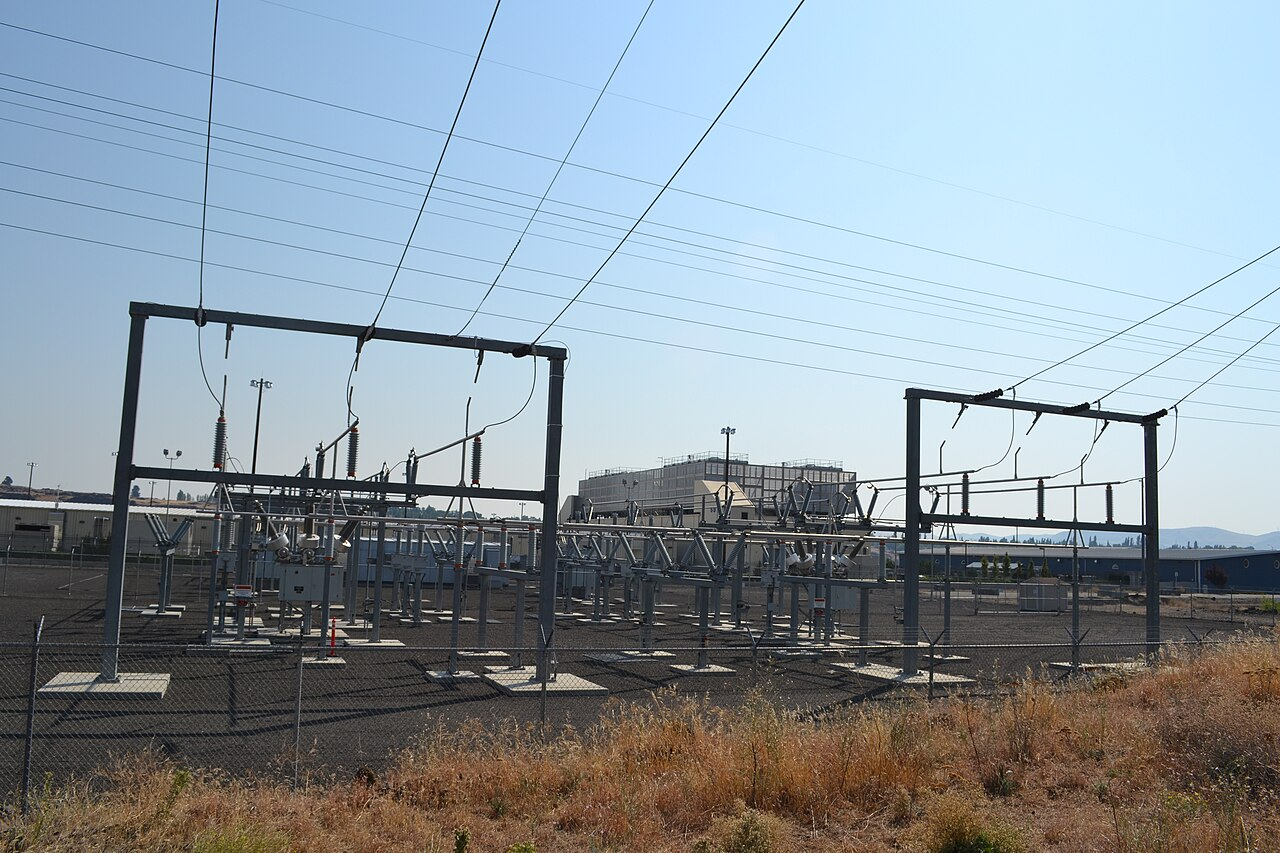
\includegraphics[height=0.46\textheight]{ch11_google_dalles_2011.jpg}\\[1mm]
\imgcap{Un centru de date Google, The Dalles, Oregon}
\imgcredit{https://commons.wikimedia.org/wiki/File:Google_Data_Center,_The_Dalles.jpg}{Foto: Visitor7 (2011); CC BY-SA 3.0; Wikimedia Commons}
\end{column}
\begin{column}{0.56\textwidth}
\begin{itemize}
    \item Corpusurile de pre-antrenare amestecă serii publice din multe domenii
    \begin{itemize}
        \item energie, transport, comerț, vreme, trafic web, finanțe și economie
        \item plus serii sintetice: amestecuri aleatoare de serii reale și serii generate din procese gaussiene (Chronos)
    \end{itemize}
    \item Scara: TimesFM a fost pre-antrenat pe circa $10^{11}$ puncte (\refDas)
    \item Pre-antrenarea se face o singură dată, de dezvoltator, pe multe procesoare grafice (GPU)
    \begin{itemize}
        \item utilizatorul doar rulează modelul: versiunile mici rulează pe un CPU obișnuit
    \end{itemize}
\end{itemize}
\end{column}
\end{columns}
\end{frame}

\begin{frame}{Recapitulare: ideea de foundation model}
\itemsize{\small}
\begin{itemize}
    \item Modelele locale, globale și de tip foundation diferă prin datele pe care se antrenează
    \item Zero-shot: ponderi fixe, doar contextul seriei noi
    \item Rezultatul este o mulțime de cuantile: o prognoză probabilistă
\end{itemize}
\end{frame}


%=============================================================================
\section{Transformer-ul, pe scurt}
%=============================================================================

\begin{frame}{Transformer-ul (Vaswani et al., 2017)}
\itemsize{\small}
\begin{columns}[T]
\begin{column}{0.34\textwidth}
\centering
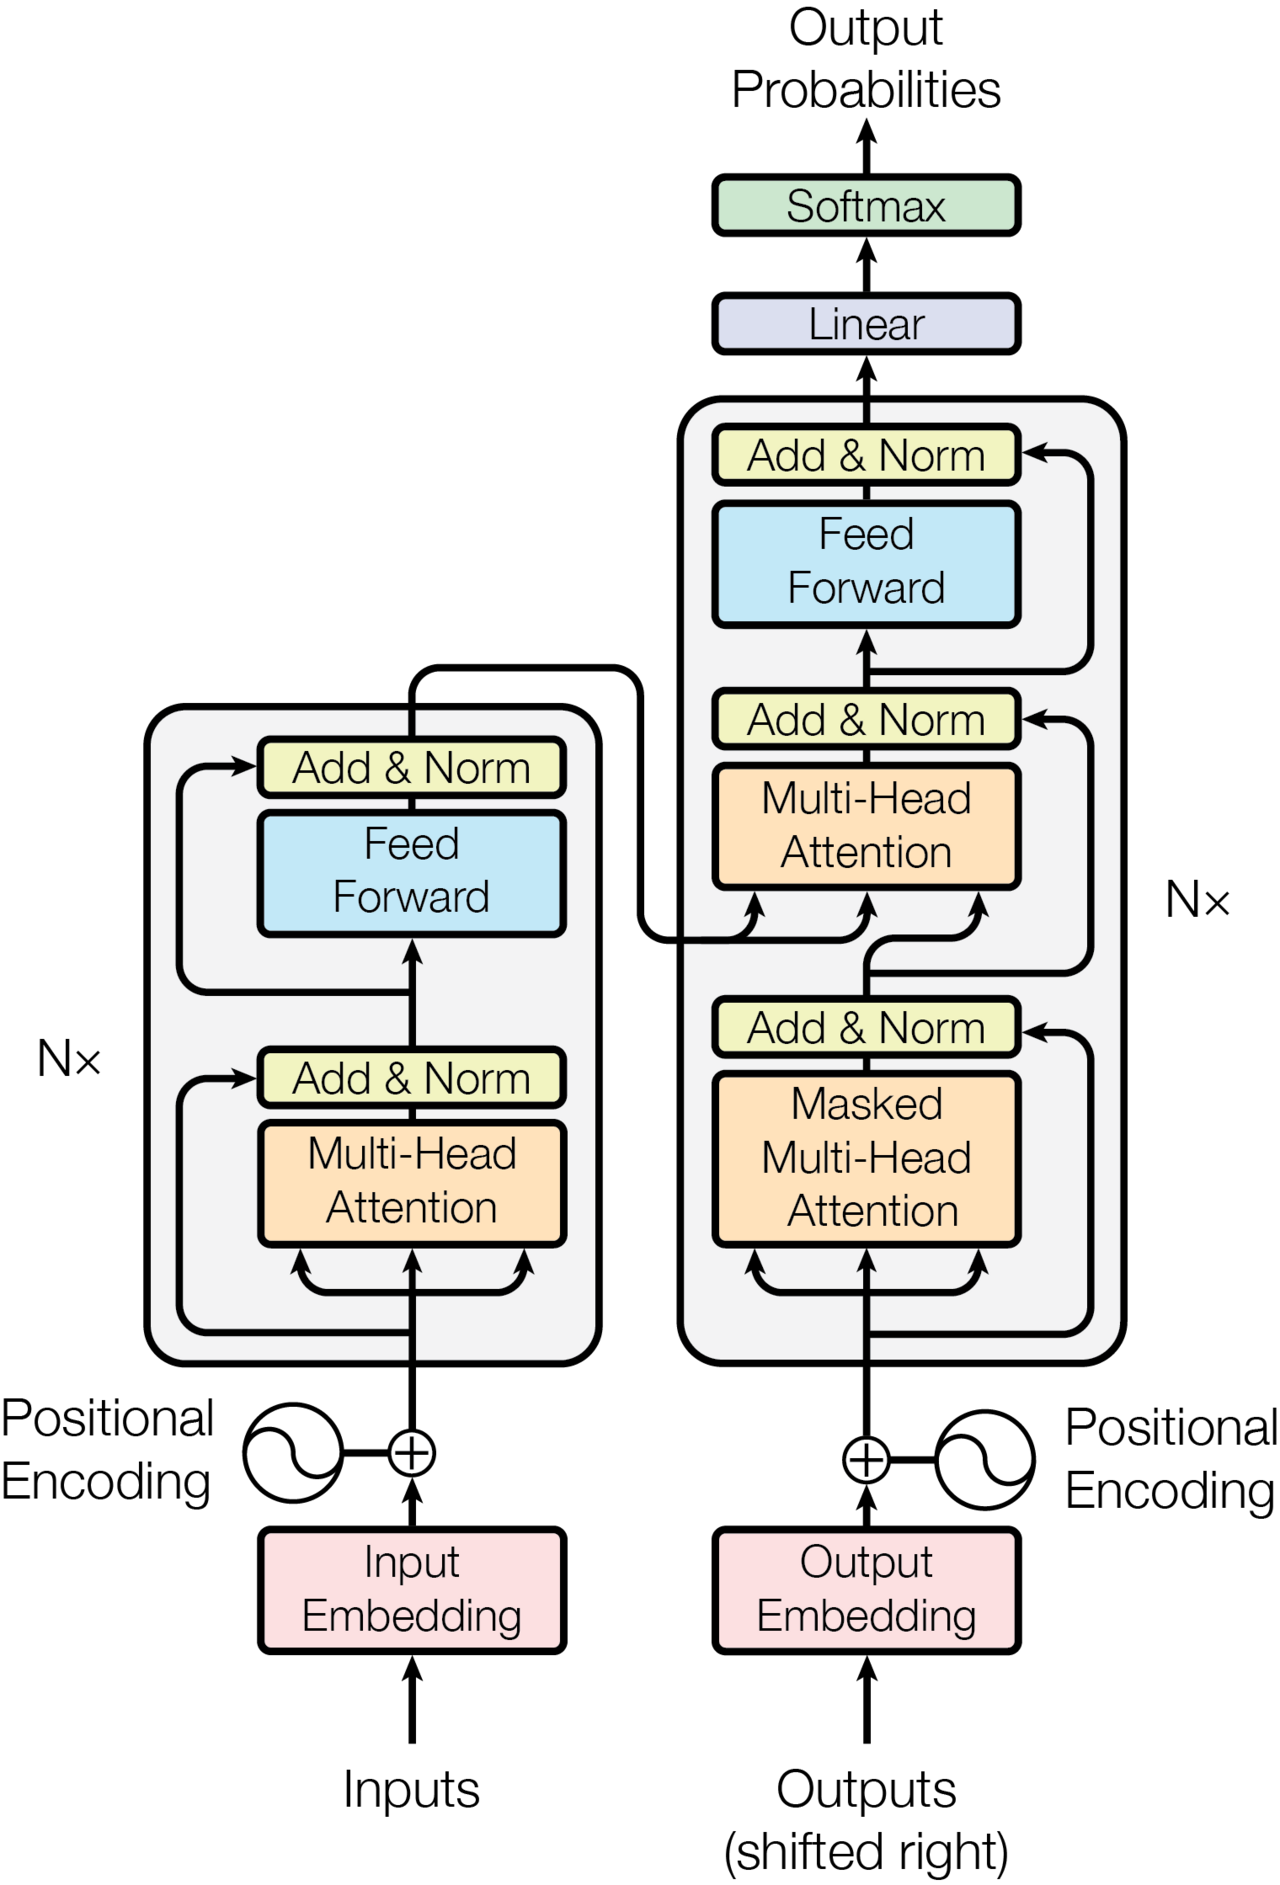
\includegraphics[height=0.62\textheight]{ch11_attention_figure_2017.png}\\[1mm]
\imgcap{Diagrama originală: encoder (stînga), decoder (dreapta)}
\imgcredit{https://commons.wikimedia.org/wiki/File:Attention_Is_All_You_Need_-_Encoder-decoder_Architecture.png}{Figura: Vaswani et al.\ (2017), Google; CC BY-SA 4.0; Wikimedia Commons}
\end{column}
\begin{column}{0.64\textwidth}
\begin{itemize}
    \item \refVaswani: o rețea pentru secvențe construită pe \textbf{atenție}, fără recurență
    \begin{itemize}
        \item creată pentru traducere; stă la baza oricărui model mare de limbaj (LLM)
    \end{itemize}
    \item Intrarea: o secvență de \textbf{tokeni}, fiecare transformat într-un vector (embedding)
    \item \textbf{Encoder-ul}: citește toată intrarea; \textbf{decoder-ul}: produce ieșirea pas cu pas
    \begin{itemize}
        \item modelele \textbf{doar cu decoder} (GPT, TimesFM, Lag-Llama) prognozează tokenul următor din toți cei anteriori
    \end{itemize}
    \item Fiecărui vector i se adaugă informația despre poziție, deoarece atenția ignoră ordinea
\end{itemize}
\end{column}
\end{columns}
\end{frame}

\begin{frame}{Self-attention (atenția asupra propriei secvențe)}
\itemsize{\footnotesize}
\begin{itemize}
    \item Fiecare vector de intrare $x_i$ produce o interogare $q_i$, o cheie $k_i$ și o valoare $v_i$ (trei transformări liniare)
    \item Ieșirea în poziția $i$: o medie ponderată a tuturor valorilor
    \begin{itemize}
        \item $\displaystyle \text{out}_i = \sum_j w_{ij} v_j, \qquad w_{ij} = \frac{\exp(q_i^\top k_j/\sqrt{d})}{\sum_l \exp(q_i^\top k_l/\sqrt{d})}$
        \item matricial: $\text{softmax}(QK^\top/\sqrt{d})\,V$; $d$ = lungimea vectorilor-cheie
    \end{itemize}
    \item Intuiția pentru serii: pasul de azi se poate uita la aceeași oră de săptămîna trecută și îi poate da o pondere mare
    \begin{itemize}
        \item ponderile sînt învățate din date, nu fixate dinainte ca decalajele unui AR($p$)
    \end{itemize}
    \item Costul: $n$ intrări cer $n^2$ comparații; un context de 2048 de valori dă circa 4 milioane
\end{itemize}
\end{frame}

\begin{frame}{Exemplu rezolvat: ponderile atenției}
\itemsize{\small}
\begin{itemize}
    \item O interogare și trei chei; scorurile $q^\top k_j/\sqrt{d}$ = 2, 1, 0; valorile $v_j$ = 10, 20, 30
    \item Pasul 1: exponențiala: $e^2$, $e^1$, $e^0$
    \item Pasul 2: împărțirea la sumă: ponderile 0{,}67; 0{,}24; 0{,}09 (au suma 1)
    \item Pasul 3: ieșirea $= \sum_j w_j v_j$ = 14{,}2
    \begin{itemize}
        \item scorul cel mai mare primește cea mai mare parte din pondere, dar fiecare valoare contribuie
    \end{itemize}
    \item Un foundation model suprapune multe astfel de straturi, fiecare cu mai multe capete de atenție
\end{itemize}
\end{frame}

\begin{frame}{Recapitulare: Transformer-ul}
\itemsize{\small}
\begin{itemize}
    \item Atenția: fiecare pas este o medie ponderată, învățată, a tuturor pașilor
    \item Construcții encoder--decoder (Chronos) și doar cu decoder (TimesFM, Lag-Llama)
    \item Costul crește cu pătratul numărului de intrări
\end{itemize}
\end{frame}


%=============================================================================
\section{De la numere la tokeni}
%=============================================================================

\begin{frame}{Problema: un model de limbaj citește cuvinte, o serie are numere}
\itemsize{\small}
\begin{itemize}
    \item Seriile diferă prin unități și niveluri: consumul în GW, un indice în jur de 100, un curs de schimb în jur de 5
    \begin{itemize}
        \item un singur model pentru toate are nevoie de o scală comună
    \end{itemize}
    \item Trei soluții folosite în practică
    \begin{itemize}
        \item \textbf{scalare + cuantizare}: fiecare valoare devine un token dintr-un vocabular fix (Chronos)
        \item \textbf{patching}: grupuri de valori consecutive devin un vector de intrare (TimesFM, Moirai, Chronos-Bolt)
        \item \textbf{cifrele ca text}: un LLM general citește numerele ca șiruri de caractere (\refGruver)
    \end{itemize}
    \item În toate cazurile, prognozele se transformă înapoi în unitățile inițiale
\end{itemize}
\end{frame}

\begin{frame}{Scalarea prin medie și cuantizarea (Chronos)}
\itemsize{\footnotesize}
\begin{itemize}
    \item \textbf{Scalarea prin medie}: $\tilde x_t = x_t / s$, cu $s = \frac{1}{C}\sum_{t=1}^{C} |x_t|$
    \begin{itemize}
        \item contextul scalat are valori de ordinul unității, oricare ar fi unitățile
    \end{itemize}
    \item \textbf{Cuantizarea}: intervalul $[-15, 15]$ este împărțit în 4093 de intervale egale; tokenul lui $\tilde x_t$ este numărul celui mai apropiat centru
    \begin{itemize}
        \item lățimea unui interval 0{,}0073; plus tokeni speciali (completare, sfîrșit de secvență)
    \end{itemize}
    \item Antrenarea: un model de limbaj (T5) învață să prognozeze tokenul următor, cu pierderea cross-entropy
    \begin{itemize}
        \item prognoza: se eșantionează multe traiectorii de tokeni, se transformă în valori ($\times s$), se citesc cuantilele
    \end{itemize}
    \item Limita: valorile scalate în afara intervalului $[-15, 15]$ nu pot fi produse
\end{itemize}
\end{frame}

\begin{frame}{Exemplu rezolvat: scalarea și tokenii}
\itemsize{\small}
\begin{itemize}
    \item Contextul: rata șomajului din România (\%, ajustată sezonier, Eurostat), martie 2026--august 2026
    \begin{itemize}
        \item $x$ = 6{,}5; 6{,}8; 6{,}7; 6{,}8; 6{,}4; 6{,}4
    \end{itemize}
    \item Pasul 1: scala $s$ = media lui $|x_t|$ = 6{,}60
    \item Pasul 2: valorile scalate $x_t/s$ = 0{,}985; 1{,}030; 1{,}015; 1{,}030; 0{,}970; 0{,}970
    \item Pasul 3: cele mai apropiate centre (de la 0 la 4092): tokenii 2180, 2187, 2184, 2187, 2178, 2178
    \begin{itemize}
        \item valorile egale dau tokeni egali; o variație de 0,1 puncte mută tokenul cu mai multe intervale
    \end{itemize}
    \item Modelul nu vede niciodată nivelul de 6,6\%: doar forma relativă la scală
\end{itemize}
\end{frame}

\begin{frame}{Scalarea și cuantizarea pe date reale}
\itemsize{\footnotesize}
\begin{center}
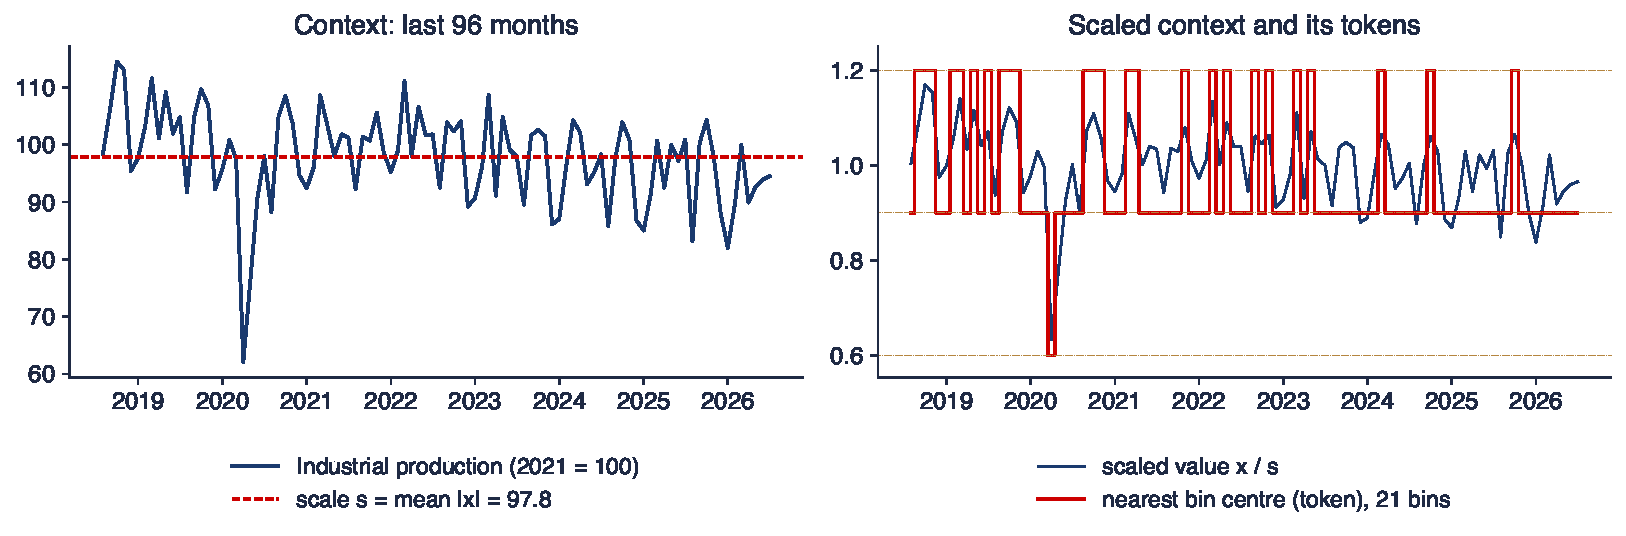
\includegraphics[width=0.97\textwidth,height=0.62\textheight,keepaspectratio]{tsa_ch11_tokens.pdf}
\end{center}
\vspace{-0.25cm}
\begin{itemize}
    \item Producția industrială a României (Eurostat, 2021 = 100), ultimele 96 de luni; scala $s$ = 97{,}8
    \item Dreapta: contextul scalat și tokenii lui pe o grilă grosieră de 21 de intervale (Chronos folosește 4093)
\end{itemize}
\quantlet{TSA\_ch11\_tokens\_scores}{\qlurl{TSA_ch11_tokens_scores}}
\end{frame}

\begin{frame}{Interpretarea tokenilor}
\itemsize{\small}
\begin{itemize}
    \item După scalare, toate valorile sînt între 0{,}63 și 1{,}17: cîteva procente din intervalul $[-15, 15]$
    \item Pe grila grosieră, cele 96 de luni folosesc doar 3 tokeni: căderea din aprilie 2020 (carantina) este un token separat
    \item Cu 4093 de intervale, grila este suficient de fină pentru a păstra forma sezonieră
    \item O valoare extremă mărește $s$ și micșorează toate celelalte valori scalate: valorile aberante din context contează
\end{itemize}
\end{frame}

\begin{frame}{Patching-ul}
\itemsize{\small}
\begin{itemize}
    \item \textbf{Patch}: un bloc de $P$ valori consecutive, transformat într-un vector de intrare de o rețea mică
    \begin{itemize}
        \item PatchTST (\refNie): „o serie de timp valorează cît 64 de cuvinte”
    \end{itemize}
    \item Două avantaje
    \begin{itemize}
        \item mai puține intrări: 2048 de valori cu $P = 16$ dau 128 de patch-uri, deci atenția cere $128^2$ în loc de $2048^2$ comparații
        \item fiecare intrare poartă o formă locală (o pantă, un vîrf), nu un singur număr zgomotos
    \end{itemize}
    \item Folosit de TimesFM (patch-uri de intrare de 32), Moirai (mărimea patch-ului după frecvență), Chronos-Bolt și Chronos-2 (16)
    \begin{itemize}
        \item și ieșirea poate fi un patch întreg de valori viitoare, ceea ce este mai rapid decît token cu token
    \end{itemize}
\end{itemize}
\end{frame}

\begin{frame}{Patching-ul consumului de energie electrică al României}
\itemsize{\footnotesize}
\begin{center}
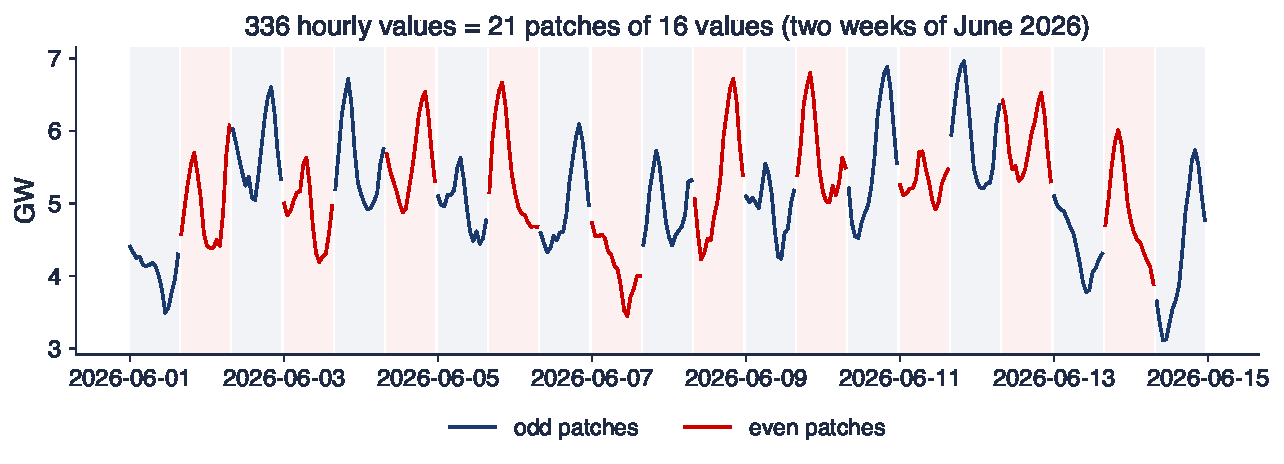
\includegraphics[width=0.97\textwidth,height=0.62\textheight,keepaspectratio]{tsa_ch11_patching.pdf}
\end{center}
\vspace{-0.25cm}
\begin{itemize}
    \item 336 de valori orare (două săptămîni din iunie 2026, ENTSO-E), împărțite în 21 de patch-uri de cîte 16 valori
\end{itemize}
\quantlet{TSA\_ch11\_tokens\_scores}{\qlurl{TSA_ch11_tokens_scores}}
\end{frame}

\begin{frame}{Interpretarea patching-ului}
\itemsize{\small}
\begin{itemize}
    \item O zi are 24 de ore, deci un patch de 16 acoperă două treimi dintr-o zi: patch-urile nu se aliniază cu ciclul zilnic
    \item Atenția leagă patch-urile: creșterea de dimineață de luni poate fi pusă în legătură cu cea de lunea trecută
    \item Un ciclu săptămînal (168 de ore) este vizibil doar dacă contextul acoperă cel puțin o săptămînă: 11 patch-uri
\end{itemize}
\end{frame}

\begin{frame}{Recapitulare: de la numere la tokeni}
\itemsize{\small}
\begin{itemize}
    \item Scalarea prin medie elimină unitățile; cuantizarea transformă valorile în tokeni (Chronos)
    \item Patching-ul grupează valorile: secvențe mai scurte, forme locale
    \item Prognoza se transformă înapoi în unitățile inițiale
\end{itemize}
\end{frame}


%=============================================================================
\section{Principalele familii de modele}
%=============================================================================

\begin{frame}{Chronos, Chronos-Bolt și Chronos-2 (Amazon)}
\itemsize{\footnotesize}
\begin{columns}[T]
\begin{column}{0.32\textwidth}
\centering
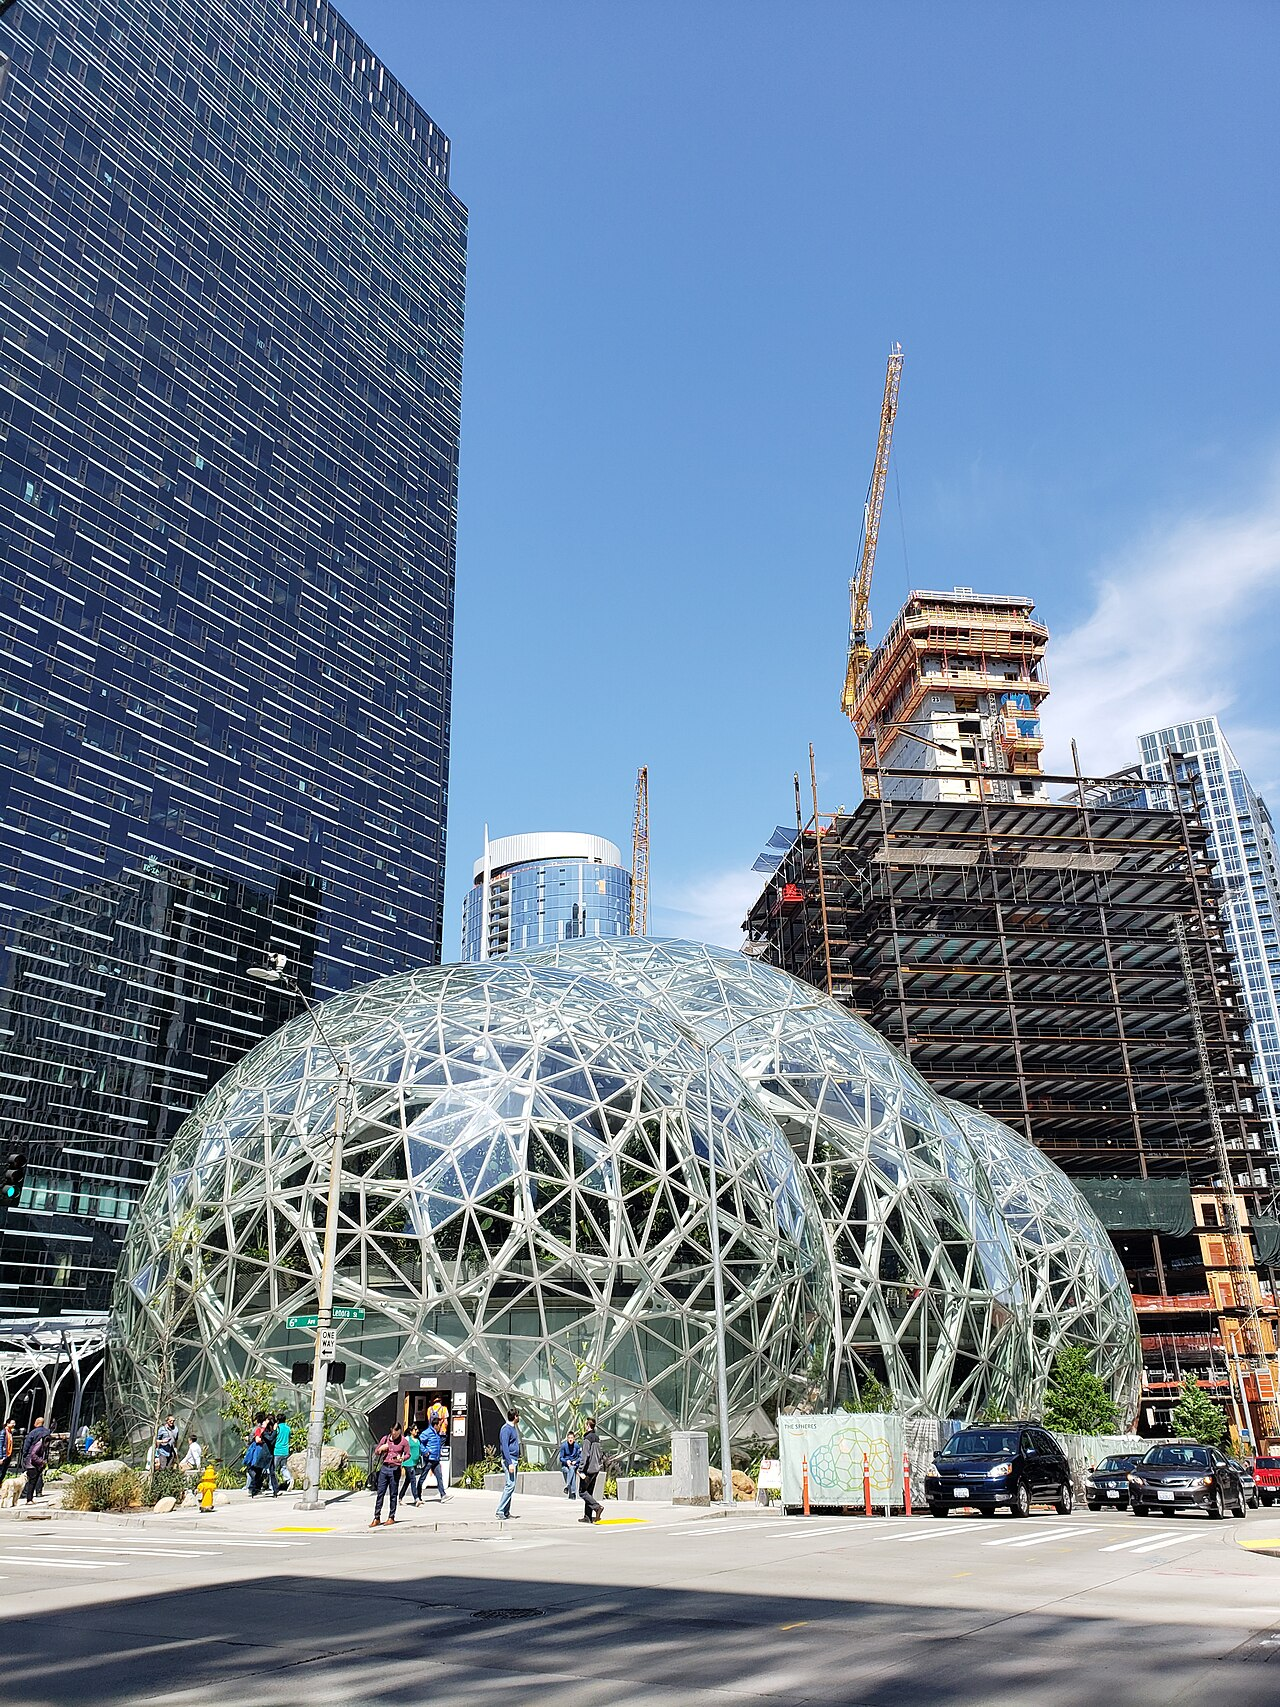
\includegraphics[height=0.62\textheight]{ch11_amazon_spheres_2018.jpg}\\[1mm]
\imgcap{Amazon Spheres, Seattle}
\imgcredit{https://commons.wikimedia.org/wiki/File:Amazon_Spheres_2018.jpg}{Foto: Andy Li (2018); CC0; Wikimedia Commons}
\end{column}
\begin{column}{0.66\textwidth}
\begin{itemize}
    \item \textbf{Chronos} (\refAnsari): T5 encoder--decoder pe valori scalate și cuantizate; eșantionează traiectorii de tokeni
    \item \textbf{Chronos-Bolt} (noiembrie 2024): patch-uri de 16 valori și ieșirea directă a cuantilelor 0,1, \dots, 0,9
    \begin{itemize}
        \item dimensiunile folosite aici: tiny, 9 milioane, și small, 48 de milioane de parametri; context de pînă la 2048 de valori
    \end{itemize}
    \item \textbf{Chronos-2} (\refAnsariB, octombrie 2025): 119 milioane de parametri, 21 de niveluri de cuantile, covariate și grupuri de serii înrudite
    \item Ponderi deschise (licența Apache-2.0); pachetul Python \texttt{chronos-forecasting}; toate rulează pe un CPU
\end{itemize}
\end{column}
\end{columns}
\end{frame}

\begin{frame}{TimesFM (Google) și Lag-Llama}
\itemsize{\footnotesize}
\begin{itemize}
    \item \textbf{TimesFM} (\refDas): Transformer doar cu decoder, patch-uri de intrare de 32 și de ieșire de 128 de valori
    \begin{itemize}
        \item pre-antrenat pe serii reale (Google Trends, accesări de pagini Wikipedia) și sintetice; circa 200 de milioane de parametri
        \item ponderi deschise (Apache-2.0); versiunile ulterioare adaugă ieșiri cuantile
    \end{itemize}
    \item \textbf{Lag-Llama} (\refRasul): doar cu decoder, construit pe arhitectura Llama a modelelor de limbaj
    \begin{itemize}
        \item intrările: valori întîrziate alese după frecvență (de exemplu 7 zile, 12 luni, 24 de ore) plus variabile de calendar
        \item ieșirea: parametrii unei distribuții Student-$t$ pentru pasul următor; eșantionarea dă traiectorii
        \item mic și deschis (Apache-2.0); gîndit pentru fine-tuning
    \end{itemize}
\end{itemize}
\end{frame}

\begin{frame}{Moirai (Salesforce) și TimeGPT}
\itemsize{\footnotesize}
\begin{columns}[T]
\begin{column}{0.3\textwidth}
\centering
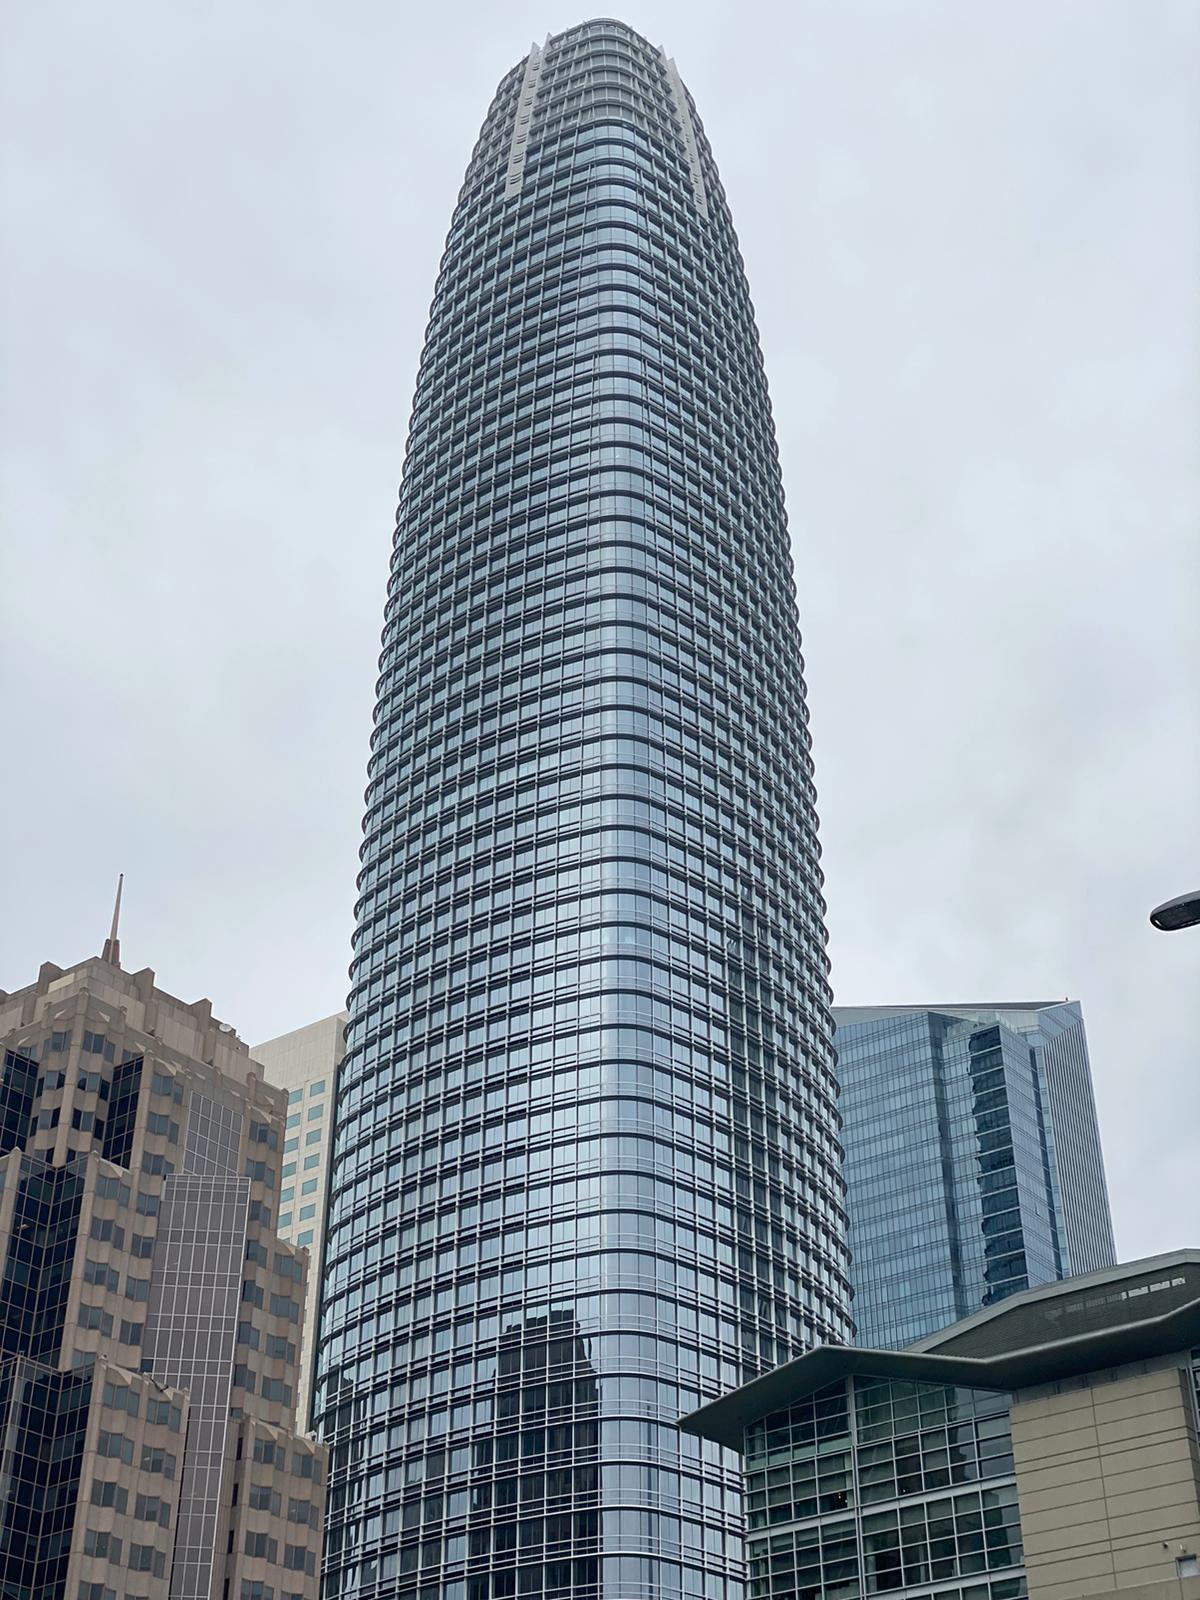
\includegraphics[height=0.62\textheight]{ch11_salesforce_tower_2020.jpg}\\[1mm]
\imgcap{Salesforce Tower, San Francisco}
\imgcredit{https://commons.wikimedia.org/wiki/File:Salesforce_Tower_2020.jpg}{Foto: Saggittarius A (2020); CC BY-SA 4.0; Wikimedia Commons}
\end{column}
\begin{column}{0.68\textwidth}
\begin{itemize}
    \item \textbf{Moirai} (\refWoo): model de prognoză „universal”
    \begin{itemize}
        \item orice număr de variabile într-o singură secvență; mărimea patch-ului aleasă după frecvență
        \item ieșirea: un amestec de distribuții; corpusul LOTSA, circa 27 de miliarde de observații
        \item ponderi deschise, cu licență necomercială (CC BY-NC 4.0)
    \end{itemize}
    \item \textbf{TimeGPT} (\refGarza): model închis, disponibil doar printr-un API cu plată
    \begin{itemize}
        \item ponderile și datele de antrenare nu pot fi inspectate; versiunea se poate schimba; datele pleacă de pe calculatorul dumneavoastră
        \item nu îl folosim în acest curs: rezultatele nu ar putea fi reproduse
    \end{itemize}
\end{itemize}
\end{column}
\end{columns}
\end{frame}

\begin{frame}{Familiile, una lîngă alta}
\itemsize{\footnotesize}
\begin{center}
\scriptsize
\begin{tabular}{lllll}
\toprule
\textbf{Model} & \textbf{Arhitectura} & \textbf{Intrarea} & \textbf{Ieșirea} & \textbf{Acces} \\
\midrule
Chronos (2024) & encoder--decoder (T5) & tokeni (intervale) & traiectorii eșantionate & Apache-2.0 \\
Chronos-Bolt (2024) & encoder--decoder & patch-uri de 16 & 9 cuantile & Apache-2.0 \\
Chronos-2 (2025) & encoder & patch-uri + covariate & 21 de cuantile & Apache-2.0 \\
TimesFM (2024) & decoder & patch-uri de 32 & patch-uri de 128 & Apache-2.0 \\
Moirai (2024) & encoder & patch-uri, orice variabile & amestec & CC BY-NC 4.0 \\
Lag-Llama (2023) & decoder (Llama) & valori întîrziate & Student-$t$ & Apache-2.0 \\
TimeGPT (2023) & nepublicată & -- & puncte, intervale & API cu plată \\
\bottomrule
\end{tabular}
\end{center}
\begin{itemize}
    \item O altă direcție dă cifrele unor LLM-uri generale (\refGruver); \refTan{} arată că partea de model de limbaj adaugă cost, dar nu și precizie
\end{itemize}
\end{frame}

\begin{frame}{Recapitulare: familiile de modele}
\itemsize{\small}
\begin{itemize}
    \item Chronos: tokeni; Chronos-Bolt și Chronos-2: patch-uri și cuantile directe
    \item TimesFM și Lag-Llama: doar cu decoder; Moirai: orice număr de variabile
    \item Ponderile deschise fac rezultatele reproductibile; un API cu plată, nu
\end{itemize}
\end{frame}


%=============================================================================
\section{Prognozele probabiliste și scorurile lor}
%=============================================================================

\begin{frame}{Prognozele cuantile}
\itemsize{\small}
\begin{itemize}
    \item O \textbf{prognoză probabilistă} dă distribuția lui $y_{T+h}$, condiționată de datele pînă la $T$
    \begin{itemize}
        \item foundation models o raportează prin cuantile $\hat q_\tau$ la nivelurile $\tau = 0{,}1, \dots, 0{,}9$
    \end{itemize}
    \item Prognoza punctuală: mediana $\hat q_{0,5}$
    \item Intervalul central de 80\%: $[\hat q_{0,1}, \hat q_{0,9}]$; un \textbf{fan chart} desenează mai multe astfel de benzi
    \item Două calități de verificat
    \begin{itemize}
        \item \textbf{calibrarea}: intervalul de 80\% conține circa 80\% din valorile observate
        \item \textbf{precizia} (sharpness): dintre prognozele calibrate, cea mai îngustă este mai bună (\refGR)
    \end{itemize}
    \item Pentru ETS și ARIMA folosim cuantilele distribuției Normale, $\hat y_{T+h} + z_\tau \hat\sigma_h$
\end{itemize}
\end{frame}

\begin{frame}{Pierderea pinball și CRPS}
\itemsize{\footnotesize}
\begin{itemize}
    \item Pierderea \textbf{pinball} (cuantilă) a lui $\hat q_\tau$ pentru valoarea observată $y$
    \begin{itemize}
        \item $L_\tau(y, \hat q_\tau) = \tau\,(y - \hat q_\tau)$ dacă $y \ge \hat q_\tau$ și $(1 - \tau)(\hat q_\tau - y)$ altfel
        \item valoarea ei așteptată este minimă în cuantila adevărată: răsplătește cuantilele oneste
    \end{itemize}
    \item \textbf{CRPS} (scorul de probabilitate continuu pe ranguri, \refMW) al unei funcții de repartiție prognozate $F$
    \begin{itemize}
        \item $\text{CRPS}(F, y) = \int (F(z) - \mathbf{1}\{z \ge y\})^2\,dz = 2\int_0^1 L_\tau(y, F^{-1}(\tau))\,d\tau$
        \item în unitățile lui $y$; pentru o prognoză punctuală este $|y - \hat y|$: CRPS generalizează MAE
    \end{itemize}
    \item \textbf{WQL} (pierderea cuantilă ponderată): CRPS aproximat cu cele 9 niveluri și împărțit la $\sum |y|$
    \begin{itemize}
        \item $\text{WQL} = \frac{1}{9}\sum_{\tau}\frac{2\sum_t L_\tau(y_t, \hat q_{\tau,t})}{\sum_t |y_t|}$: fără unități, folosit de Chronos și de GIFT-Eval
    \end{itemize}
\end{itemize}
\end{frame}

\begin{frame}{Pierderea pinball și CRPS}
\itemsize{\footnotesize}
\begin{center}
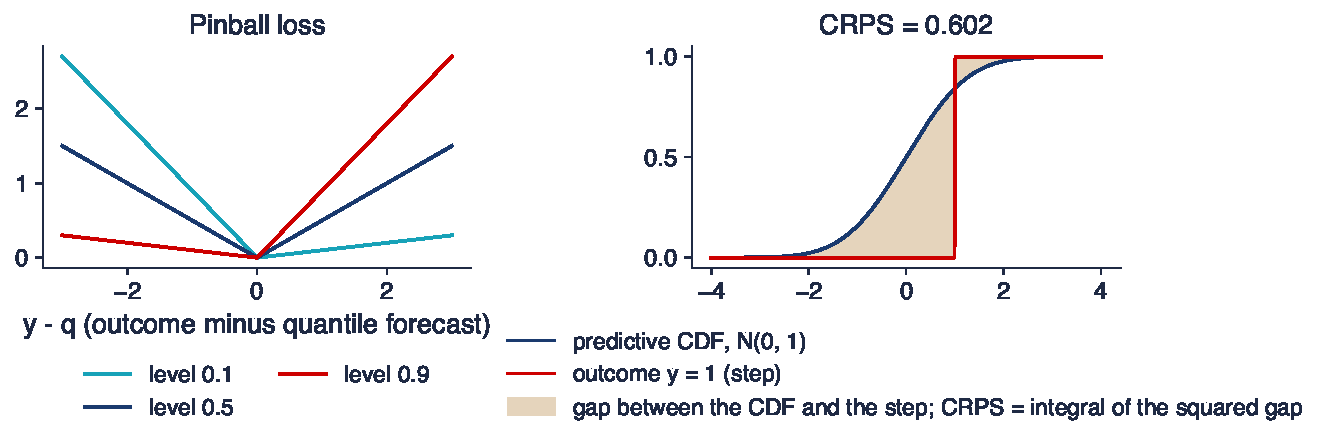
\includegraphics[width=0.97\textwidth,height=0.58\textheight,keepaspectratio]{tsa_ch11_scores.pdf}
\end{center}
\vspace{-0.25cm}
\begin{itemize}
    \item Stînga: $L_\tau$ în funcție de $y - \hat q$ pentru $\tau$ = 0,1; 0,5; 0,9. Dreapta: prognoza N(0, 1), valoarea observată $y = 1$
\end{itemize}
\quantlet{TSA\_ch11\_tokens\_scores}{\qlurl{TSA_ch11_tokens_scores}}
\end{frame}

\begin{frame}{Interpretarea scorurilor}
\itemsize{\small}
\begin{itemize}
    \item La $\tau = 0{,}9$, o valoare peste cuantilă costă de 9 ori mai mult decît una sub ea: cuantila de 0,9 ar trebui depășită doar în 10\% din cazuri
    \item La $\tau = 0{,}5$, pierderea este jumătate din eroarea absolută: mediana este evaluată ca o prognoză punctuală
    \item CRPS pentru N(0, 1): 0{,}234 dacă $y = 0$, 0{,}602 dacă $y = 1$; N(0, 4) în $y = 1$ dă 0{,}663: o bandă mai largă este penalizată chiar dacă acoperă valoarea
    \item CRPS răsplătește în același timp calibrarea și precizia
\end{itemize}
\end{frame}

\begin{frame}{Exemplu rezolvat: pierderile pinball}
\itemsize{\small}
\begin{itemize}
    \item Prognoza ratei șomajului pentru luna viitoare: $\hat q_{0,1}$ = 6{,}5, $\hat q_{0,5}$ = 7{,}0, $\hat q_{0,9}$ = 7{,}6; valoarea observată $y$ = 7{,}2
    \item $\tau = 0{,}1$: $y$ este deasupra, pierderea $0{,}1 \cdot (7{,}2 - 6{,}5)$ = 0{,}07
    \item $\tau = 0{,}5$: $y$ este deasupra, pierderea $0{,}5 \cdot (7{,}2 - 7{,}0)$ = 0{,}10
    \item $\tau = 0{,}9$: $y$ este dedesubt, pierderea $(1 - 0{,}9) \cdot (7{,}6 - 7{,}2)$ = 0{,}04
    \item CRPS aproximat cu aceste trei niveluri: $\frac{2}{3}$ (suma pierderilor) = 0{,}140 puncte procentuale
    \begin{itemize}
        \item valoarea observată este în intervalul de 80\% [6,5; 7,6]: indicatorul de acoperire este 1
    \end{itemize}
\end{itemize}
\end{frame}

\begin{frame}{Precizia punctuală și acoperirea}
\itemsize{\footnotesize}
\begin{itemize}
    \item \textbf{MASE} (\refHK): MAE al prognozei împărțit la MAE în eșantion al prognozei sezoniere naive
    \begin{itemize}
        \item $\text{MASE} = \dfrac{\frac1h\sum_{j=1}^{h}|y_{T+j} - \hat y_{T+j}|}{\frac{1}{T-m}\sum_{t=m+1}^{T}|y_t - y_{t-m}|}$; sub 1: mai bun decît prognoza sezonieră naivă în eșantion
        \item exemplu: MAE 0{,}30, MAE naiv în eșantion 0{,}25, deci MASE = 1{,}2
    \end{itemize}
    \item \textbf{Acoperirea}: proporția valorilor observate din $[\hat q_{0,1}, \hat q_{0,9}]$; ținta este 80\%
    \begin{itemize}
        \item 7 din 10 în interval înseamnă 70\%: intervale puțin prea înguste
    \end{itemize}
    \item \textbf{Scorurile relative}: MASE sau WQL al unui model împărțit la cel al prognozei sezoniere naive, pe aceleași origini
    \begin{itemize}
        \item mediate pe serii cu media geometrică, astfel încît 2 și 0,5 se compensează
    \end{itemize}
\end{itemize}
\end{frame}

\begin{frame}{Recapitulare: scorurile}
\itemsize{\small}
\begin{itemize}
    \item Pierderea pinball pentru fiecare cuantilă; CRPS pentru întreaga distribuție; WQL ca aproximare scalată
    \item MASE pentru mediană; acoperirea pentru calibrare
    \item Raportați scorurile relativ la prognoza sezonieră naivă
\end{itemize}
\end{frame}


%=============================================================================
\section{Prognoze zero-shot pe date reale}
%=============================================================================

\begin{frame}{Șapte serii pentru test}
\itemsize{\footnotesize}
\begin{center}
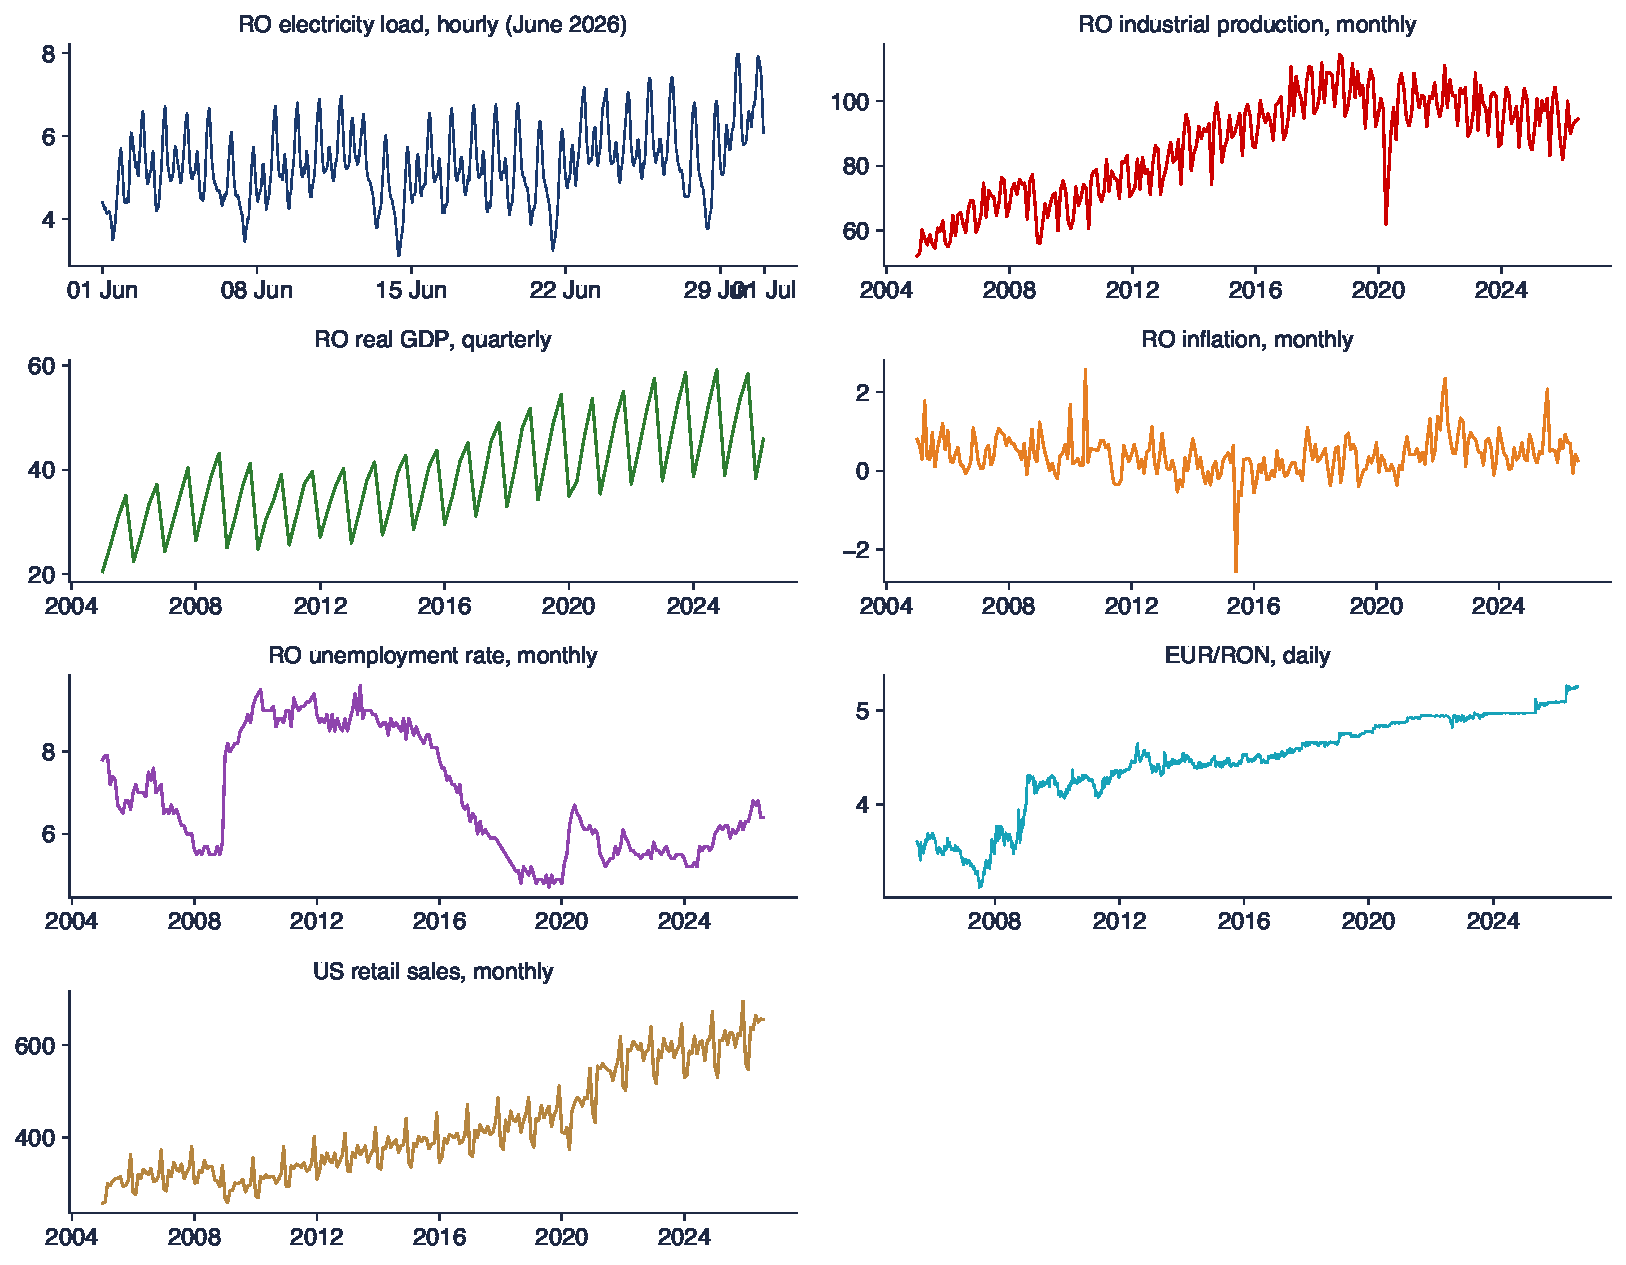
\includegraphics[width=0.97\textwidth,height=0.62\textheight,keepaspectratio]{tsa_ch11_series.pdf}
\end{center}
\vspace{-0.25cm}
\begin{itemize}
    \item Consumul orar al României (ENTSO-E); producția industrială, PIB-ul real (neajustat sezonier), inflația IAPC, șomajul în România (Eurostat); EUR/RON (BNR); vînzările cu amănuntul din SUA (FRED RSXFSN)
\end{itemize}
\quantlet{TSA\_ch11\_tokens\_scores}{\qlurl{TSA_ch11_tokens_scores}}
\end{frame}

\begin{frame}{Interpretarea celor șapte serii}
\itemsize{\small}
\begin{itemize}
    \item Sezonalitate puternică: consumul (cicluri zilnice și săptămînale), producția industrială și vînzările din SUA (anuale), PIB-ul (trimestrial)
    \item Aproape de un mers aleator: EUR/RON și rata șomajului; zgomotoasă și cu memorie scurtă: inflația lunară
    \item Rupturi: pandemia din 2020 (producția industrială, PIB-ul, vînzările); creșterea inflației din 2022
    \item Lungimi de la 126 de trimestre (PIB) la 39\,408 ore (consumul): cantități foarte diferite de context
\end{itemize}
\end{frame}

\begin{frame}{Consumul de energie electrică al României, cu 48 de ore înainte}
\itemsize{\footnotesize}
\begin{center}
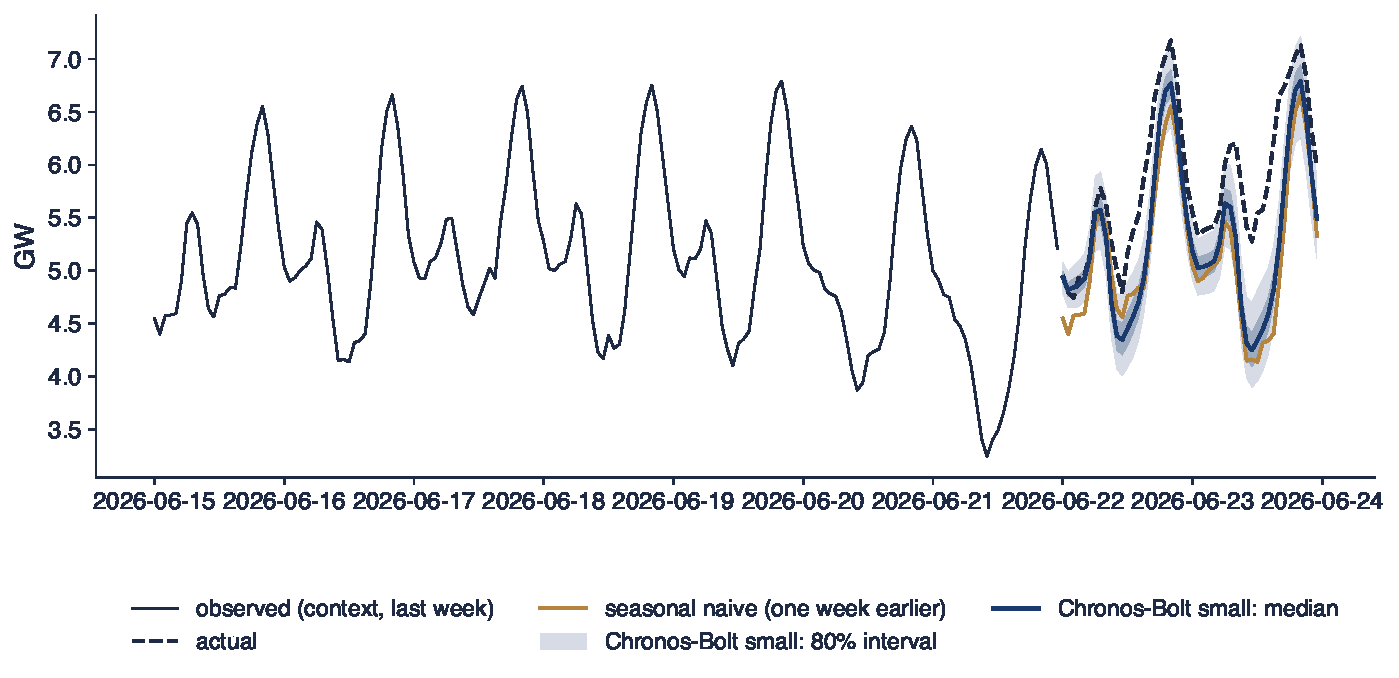
\includegraphics[width=0.97\textwidth,height=0.62\textheight,keepaspectratio]{tsa_ch11_fan_load.pdf}
\end{center}
\vspace{-0.25cm}
\begin{itemize}
    \item Chronos-Bolt small, zero-shot, context de 2048 de ore (85 de zile); originea 22 iunie 2026, ora 00:00; benzi: intervalele centrale de 50\% și 80\%
\end{itemize}
\quantlet{TSA\_ch11\_zero\_shot}{\qlurl{TSA_ch11_zero_shot}}
\end{frame}

\begin{frame}{Interpretarea prognozei consumului}
\itemsize{\small}
\begin{itemize}
    \item Modelul reproduce forma zilnică (minimul de noapte, vîrful de seară) fără nicio estimare pe această serie
    \item MASE: Chronos-Bolt 1{,}31, prognoza sezonieră naivă 1{,}61: mai bun decît repetarea săptămînii trecute
    \item Dar consumul efectiv rămîne peste prognoză toată ziua: doar 29\% din cele 48 de ore cad în banda de 80\%
    \item Modelul nu primește temperatura sau calendarul: o schimbare a vremii pe care ultimele 85 de zile nu o anunță nu poate fi anticipată
    \item O singură origine dovedește puțin: urmează testul sistematic
\end{itemize}
\end{frame}

\begin{frame}{Exemplu rezolvat: evaluarea unei ore}
\itemsize{\small}
\begin{itemize}
    \item Ora 24 a prognozei consumului (22 iunie 2026, ora 23:00): $\hat q_{0,1}$ = 5{,}18, $\hat q_{0,5}$ = 5{,}48, $\hat q_{0,9}$ = 5{,}78 GW; valoarea observată 5{,}80 GW
    \item Toate cele trei cuantile sînt sub valoarea observată, deci fiecare pierdere este $\tau\,(y - \hat q_\tau)$
    \begin{itemize}
        \item $\tau = 0{,}1$: 0{,}062; \ $\tau = 0{,}5$: 0{,}163; \ $\tau = 0{,}9$: 0{,}025 GW
    \end{itemize}
    \item Valoarea observată este peste $\hat q_{0,9}$: indicatorul de acoperire este 0 pentru această oră
    \item Mediate pe multe ore și origini, aceste pierderi dau WQL din secțiunea următoare
\end{itemize}
\end{frame}

\begin{frame}{Producția industrială a României, cu 12 luni înainte}
\itemsize{\footnotesize}
\begin{center}
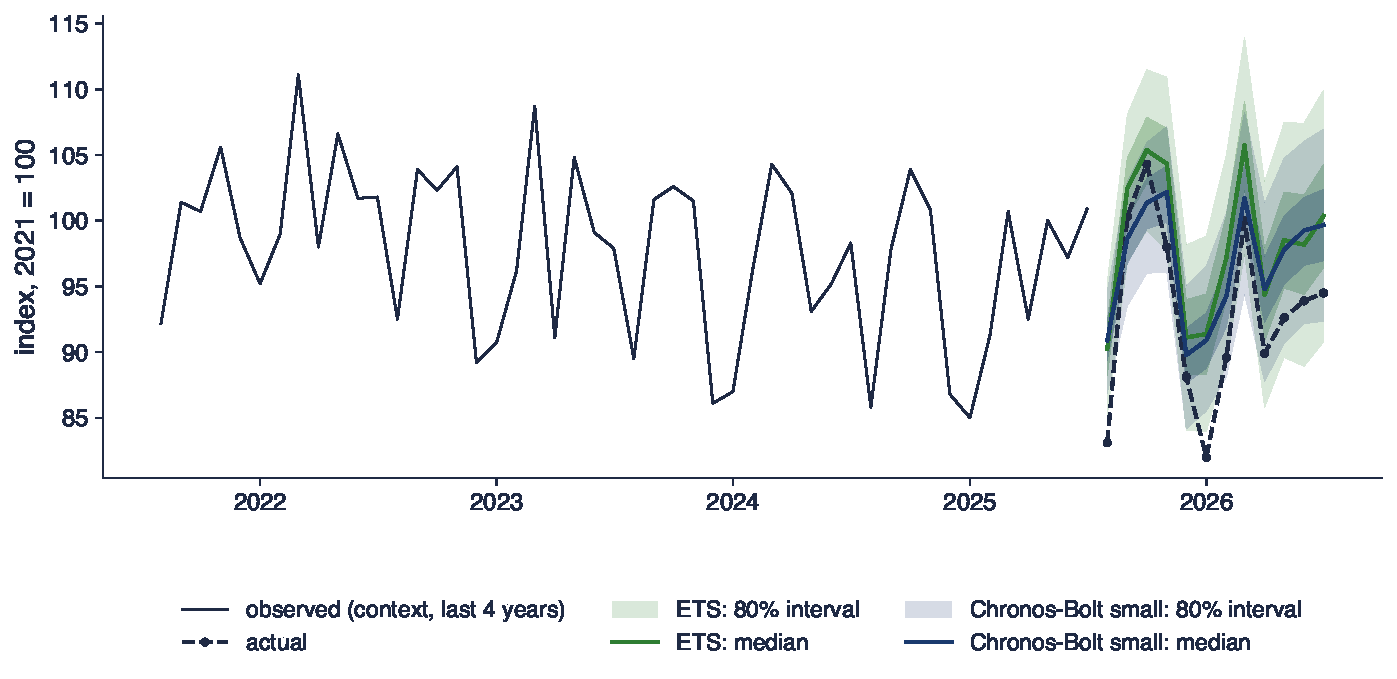
\includegraphics[width=0.97\textwidth,height=0.62\textheight,keepaspectratio]{tsa_ch11_fan_ip.pdf}
\end{center}
\vspace{-0.25cm}
\begin{itemize}
    \item Originea august 2025, prognoze pînă în iulie 2026; Chronos-Bolt small (zero-shot) și ETS (estimat pe serie), ambele cu benzi de 80\%
\end{itemize}
\quantlet{TSA\_ch11\_zero\_shot}{\qlurl{TSA_ch11_zero_shot}}
\end{frame}

\begin{frame}{Interpretarea prognozei producției industriale}
\itemsize{\small}
\begin{itemize}
    \item Ambele modele copiază tiparul sezonier (scăderile din august și decembrie) și păstrează nivelul recent
    \item MASE: Chronos-Bolt 1{,}04, ETS 1{,}20, prognoza sezonieră naivă 0{,}67: pentru această origine cîștigă cea mai simplă prognoză
    \item Producția slabă din 2026 nu este anunțată de context; benzile de 80\% acoperă 83\% (Chronos-Bolt) și 83\% (ETS) din luni
    \item Benzile Chronos-Bolt sînt mai înguste decît cele ale ETS la orizonturi lungi
\end{itemize}
\end{frame}

\begin{frame}{EUR/RON, cu 20 de zile înainte}
\itemsize{\footnotesize}
\begin{center}
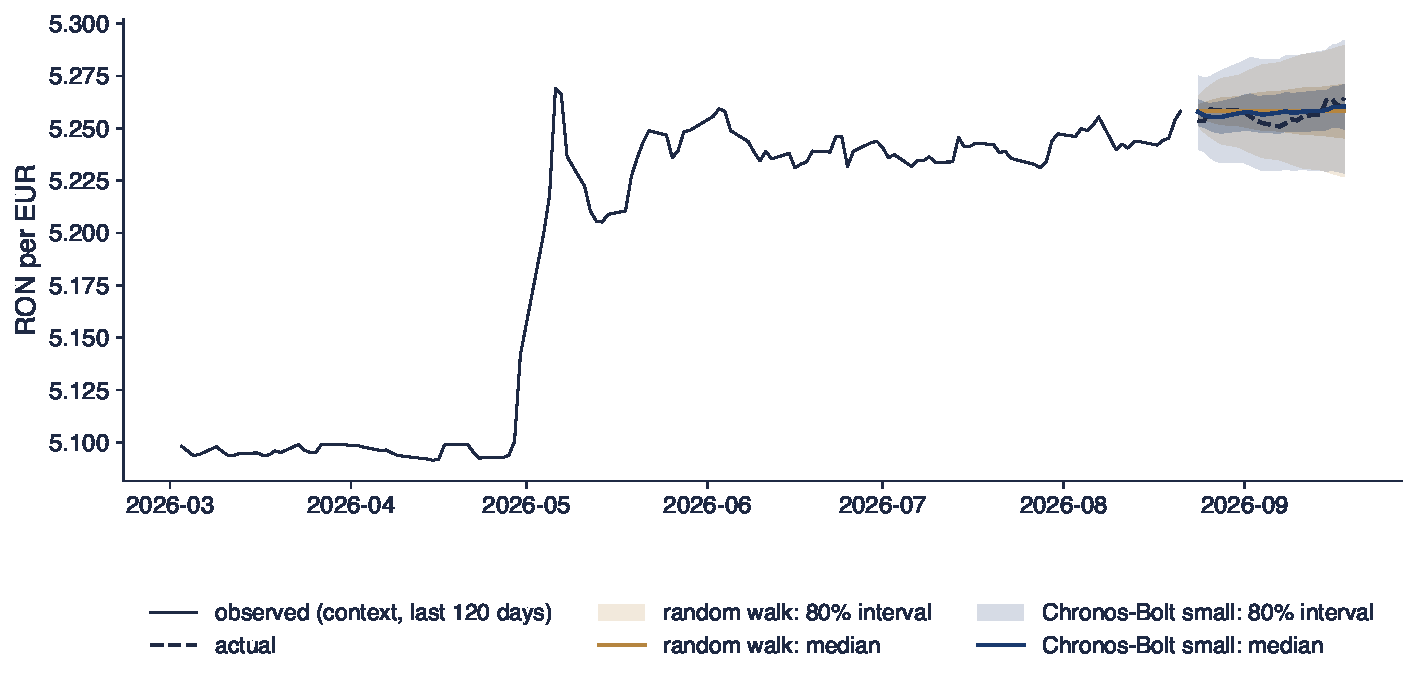
\includegraphics[width=0.97\textwidth,height=0.62\textheight,keepaspectratio]{tsa_ch11_fan_eurron.pdf}
\end{center}
\vspace{-0.25cm}
\begin{itemize}
    \item Cursul de referință BNR; originea 24 august 2026, ultima valoare dinaintea ei 5{,}2581; Chronos-Bolt small comparat cu mersul aleator cu benzi Normale
\end{itemize}
\quantlet{TSA\_ch11\_zero\_shot}{\qlurl{TSA_ch11_zero_shot}}
\end{frame}

\begin{frame}{Interpretarea prognozei EUR/RON}
\itemsize{\small}
\begin{itemize}
    \item Mediana după 20 de zile este 5{,}2604, practic ultima valoare, 5{,}2581: modelul a învățat să se comporte ca un mers aleator
    \item Lățimea benzii de 80\% la 20 de zile: 0{,}064 (Chronos-Bolt) și 0{,}063 (mersul aleator): aproape aceeași incertitudine
    \item MAE pe cele 20 de zile: 0{,}0032 față de 0{,}0035: practic egalitate
    \item Un model nu poate extrage ce trecutul nu conține: cursurile de schimb rămîn aproape imprevizibile (\tsachlink{https://danpele.github.io/Time-Series-Analysis/RO/Cursuri/capitol1_procese_stochastice_stationaritate.pdf}{Capitolul 1})
\end{itemize}
\end{frame}

\begin{frame}{Recapitulare: prognozele zero-shot}
\itemsize{\small}
\begin{itemize}
    \item Fără estimare, modelul copiază ciclurile și nivelurile din context
    \item Nu poate anticipa ce contextul nu arată (căldura, o recesiune)
    \item Pe un mers aleator întoarce un mers aleator
\end{itemize}
\end{frame}


%=============================================================================
\section{O evaluare corectă}
%=============================================================================

\begin{frame}{Protocolul testului}
\itemsize{\footnotesize}
\begin{itemize}
    \item \textbf{Origine mobilă} (\tsachlink{https://danpele.github.io/Time-Series-Analysis/RO/Cursuri/capitol4_sezonalitate_prognoza.pdf}{Capitolul 4}): la fiecare origine, fiecare model prognozează $h$ pași doar din datele pînă la origine
    \begin{itemize}
        \item consumul: $h$ = 48 de ore, origini săptămînale din iulie 2025 pînă în iunie 2026; seriile lunare: $h$ = 12, origini lunare din 2016; PIB-ul: $h$ = 4, din 2012; EUR/RON: $h$ = 20 de zile, la fiecare 20 de zile din 2016
        \item 708 origini în total; contextul: tot trecutul, cel mult 2048 de observații
    \end{itemize}
    \item \textbf{Reperele}, reestimate la fiecare origine
    \begin{itemize}
        \item prognoza sezonieră naivă (prognoza naivă pentru șomaj și EUR/RON)
        \item ETS cu trend amortizat și sezonalitate aditivă; ARIMA cu ordinele alese o singură dată după AIC, înainte de prima origine (consumul: ARMA(2,0,2) pe diferențele săptămînale)
    \end{itemize}
    \item \textbf{Foundation models}, zero-shot: Chronos-Bolt tiny și small, Chronos-2
    \item Aceleași origini, același context, același orizont, aceleași scoruri: MASE, WQL, acoperirea
\end{itemize}
\end{frame}

\begin{frame}{Rezultate: WQL relativ la prognoza sezonieră naivă}
\itemsize{\footnotesize}
\begin{center}
\scriptsize
\begin{tabular}{lcccccc}
\toprule
\textbf{Seria} & \textbf{Origini} & ETS & ARIMA & Bolt tiny & Bolt small & Chronos-2 \\
\midrule
Consumul RO (orar) & 52 & 1{,}75 & 0{,}96 & 0{,}69 & 0{,}66 & 0{,}58 \\
Producția industrială RO & 116 & 0{,}92 & 0{,}97 & 0{,}94 & 0{,}95 & 0{,}79 \\
PIB-ul real RO & 55 & 0{,}82 & 0{,}72 & 1{,}48 & 1{,}22 & 0{,}94 \\
Inflația RO & 117 & 0{,}88 & 0{,}87 & 0{,}81 & 0{,}82 & 0{,}81 \\
Șomajul RO & 117 & 1{,}00 & 0{,}99 & 1{,}03 & 0{,}99 & 0{,}96 \\
EUR/RON (zilnic) & 134 & 1{,}01 & 1{,}01 & 0{,}96 & 0{,}93 & 0{,}87 \\
Vînzările cu amănuntul SUA & 117 & 0{,}69 & 0{,}66 & 0{,}90 & 0{,}84 & 0{,}60 \\
\midrule Media geometrică & & 0{,}97 & 0{,}87 & 0{,}95 & 0{,}90 & 0{,}78 \\
\bottomrule
\end{tabular}
\end{center}
\begin{itemize}
    \item Sub 1: mai bun decît prognoza sezonieră naivă; fiecare valoare este WQL al modelului împărțit la cel al prognozei sezoniere naive pe aceleași origini
\end{itemize}
\end{frame}

\begin{frame}{MASE și WQL pe serii și modele}
\itemsize{\footnotesize}
\begin{center}
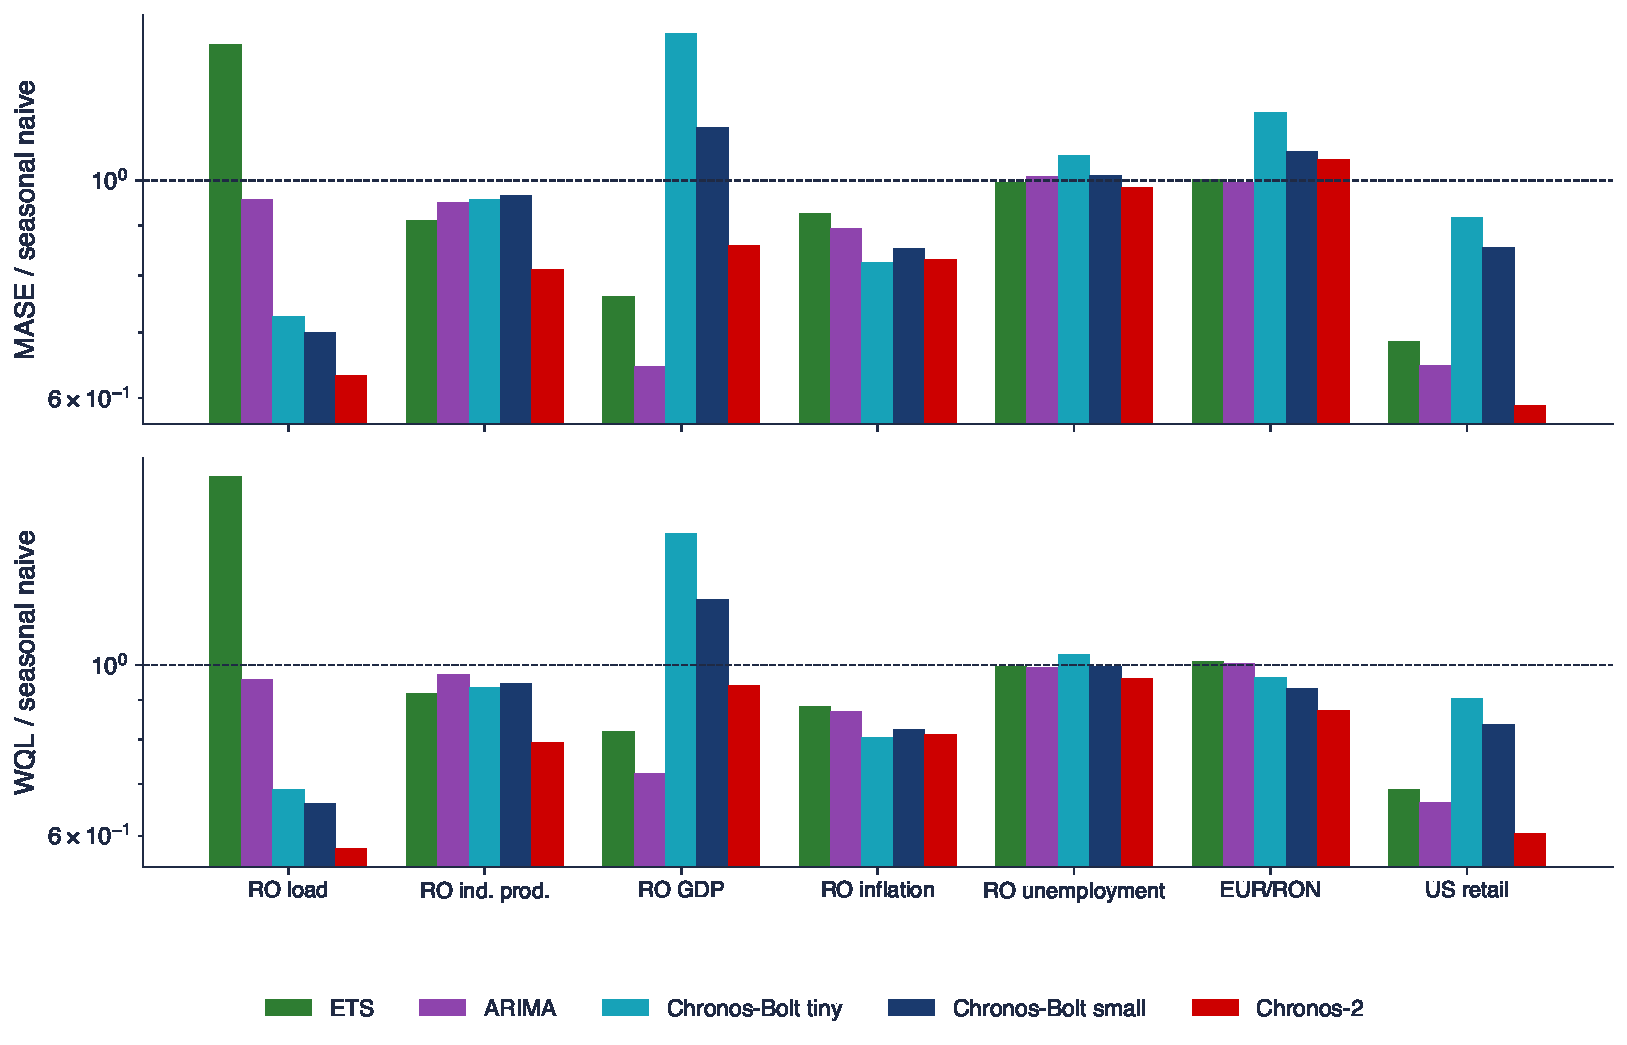
\includegraphics[width=0.97\textwidth,height=0.66\textheight,keepaspectratio]{tsa_ch11_benchmark.pdf}
\end{center}
\vspace{-0.25cm}
\begin{itemize}
    \item Rapoarte față de prognoza sezonieră naivă (scală logaritmică; linia punctată este 1)
\end{itemize}
\quantlet{TSA\_ch11\_benchmark}{\qlurl{TSA_ch11_benchmark}}
\end{frame}

\begin{frame}{Interpretarea testului}
\itemsize{\footnotesize}
\begin{itemize}
    \item Consumul orar: foundation models cîștigă clar (raportul WQL 0{,}58 pentru Chronos-2, 0{,}66 pentru Bolt small, 0{,}96 pentru ARIMA); ETS, doar cu sezonul zilnic, eșuează (1{,}75)
    \item PIB-ul României (serie trimestrială scurtă): ARIMA este cel mai bun (0{,}72); Chronos-Bolt este mai slab decît prognoza sezonieră naivă (1{,}22)
    \item Șomajul și EUR/RON: toate modelele sînt aproape de 1: nimic nu bate cu mult prognoza naivă
    \item Media geometrică a WQL: Chronos-2 0{,}78, ARIMA 0{,}87, Bolt small 0{,}90, Bolt tiny 0{,}95, ETS 0{,}97; Chronos-2 este cel mai bun pe 5 din 7 serii
    \item Un ARIMA bine specificat este la fel de bun ca foundation models mici; un cîștigător unic pe toate seriile nu există
\end{itemize}
\end{frame}

\begin{frame}{Acoperirea intervalelor de 80\%}
\itemsize{\footnotesize}
\begin{center}
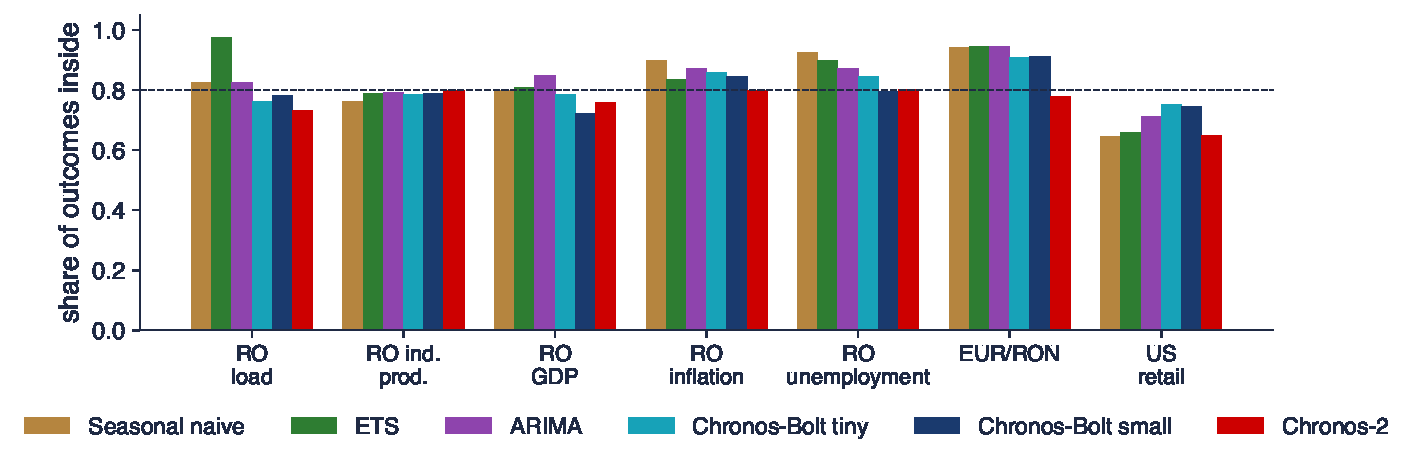
\includegraphics[width=0.97\textwidth,height=0.66\textheight,keepaspectratio]{tsa_ch11_coverage.pdf}
\end{center}
\vspace{-0.25cm}
\begin{itemize}
    \item Proporția valorilor observate din $[\hat q_{0,1}, \hat q_{0,9}]$, pe toate originile și toți pașii; linia punctată este ținta de 0,8
\end{itemize}
\quantlet{TSA\_ch11\_benchmark}{\qlurl{TSA_ch11_benchmark}}
\end{frame}

\begin{frame}{Interpretarea acoperirii}
\itemsize{\small}
\begin{itemize}
    \item Acoperirea medie: prognoza sezonieră naivă 83\%, ETS 84\%, ARIMA 84\%, Bolt small 80\%, Chronos-2 76\%
    \item Chronos-2 are cel mai bun WQL, dar intervale prea înguste: precis, dar nu complet calibrat
    \item Vînzările din SUA: fiecare model acoperă mult sub 80\% (de la 65\% pentru Chronos-2 la 75\% pentru Bolt tiny): șocul din 2020 și saltul din 2021 îi surprind pe toți
    \item Benzile ETS și ARIMA presupun erori Normale și varianță constantă: prea largi în perioadele calme, prea înguste în crize
\end{itemize}
\end{frame}

\begin{frame}{Consumul României: eroarea în funcție de orizont}
\itemsize{\footnotesize}
\begin{center}
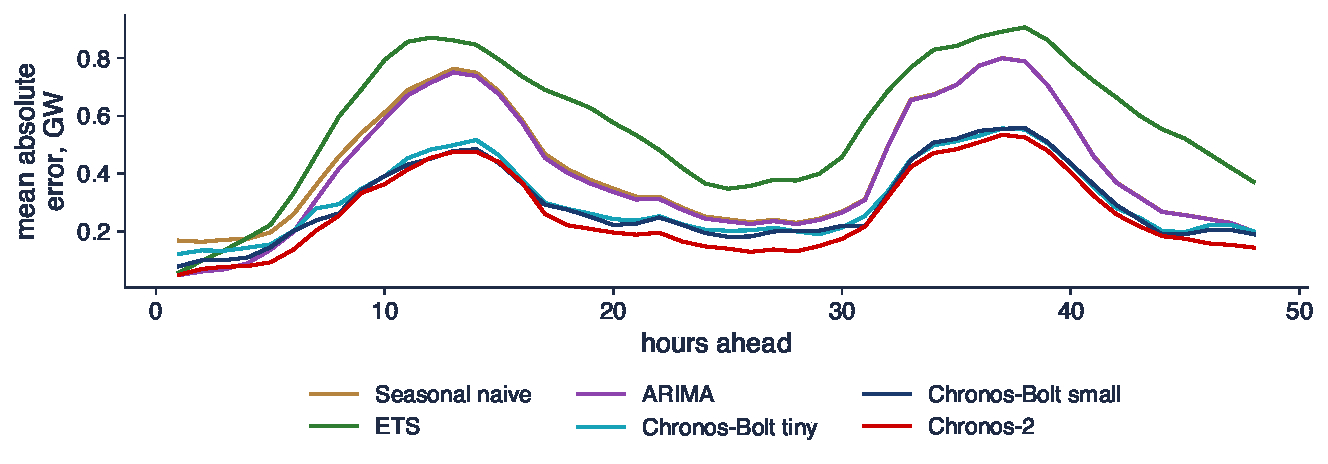
\includegraphics[width=0.97\textwidth,height=0.62\textheight,keepaspectratio]{tsa_ch11_horizon.pdf}
\end{center}
\vspace{-0.25cm}
\begin{itemize}
    \item Eroarea absolută medie (GW) a prognozei mediane pentru fiecare dintre cele 48 de ore, pe 52 de origini săptămînale
\end{itemize}
\quantlet{TSA\_ch11\_benchmark}{\qlurl{TSA_ch11_benchmark}}
\end{frame}

\begin{frame}{Interpretarea erorii în funcție de orizont}
\itemsize{\small}
\begin{itemize}
    \item Prima oră: ARIMA 0{,}05 și Chronos-2 0{,}05 GW, mult mai bine decît prognoza sezonieră naivă, 0{,}17: ultima observație contează cel mai mult
    \item După o zi, ARIMA revine la nivelul prognozei naive (0{,}24 față de 0{,}25 GW): corecția lui se stinge
    \item Chronos-2 își păstrează avantajul pe tot orizontul (0{,}14 GW la 48 de ore, față de 0{,}20)
    \item ETS este bun cîteva ore, apoi cel mai slab: un sezon zilnic nu poate reprezenta weekendul
\end{itemize}
\end{frame}

\begin{frame}{Cît context este necesar?}
\itemsize{\footnotesize}
\begin{center}
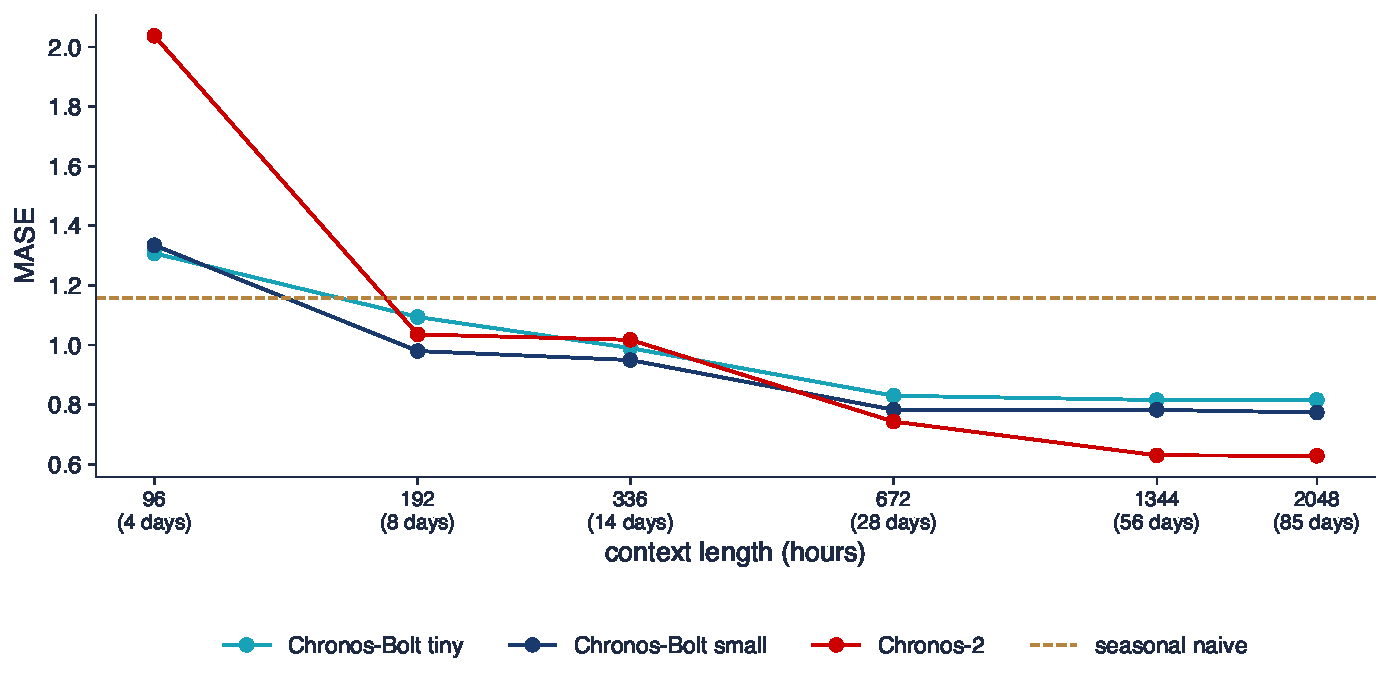
\includegraphics[width=0.97\textwidth,height=0.62\textheight,keepaspectratio]{tsa_ch11_context.pdf}
\end{center}
\vspace{-0.25cm}
\begin{itemize}
    \item MASE pentru consumul României cu contexte de 96 pînă la 2048 de ore; 26 de origini săptămînale (ultima jumătate de an); linia punctată este prognoza sezonieră naivă
\end{itemize}
\quantlet{TSA\_ch11\_context\_contamination}{\qlurl{TSA_ch11_context_contamination}}
\end{frame}

\begin{frame}{Interpretarea lungimii contextului}
\itemsize{\small}
\begin{itemize}
    \item Cu 96 de ore (4 zile), fiecare model este mai slab decît prognoza sezonieră naivă: Chronos-Bolt small 1{,}33, Chronos-2 2{,}04, naiv 1{,}16
    \item De la 192 de ore (peste o săptămînă), ciclul săptămînal intră în context și eroarea scade
    \item Chronos-2 se îmbunătățește pînă la 1344 de ore (0{,}63); Chronos-Bolt se stabilizează de la 672 de ore (0{,}78)
    \item Regula: dați modelului mai multe cicluri sezoniere complete; un model zero-shot doar repetă ce vede
\end{itemize}
\end{frame}

\begin{frame}{Dimensiunea și precizia}
\itemsize{\footnotesize}
\begin{center}
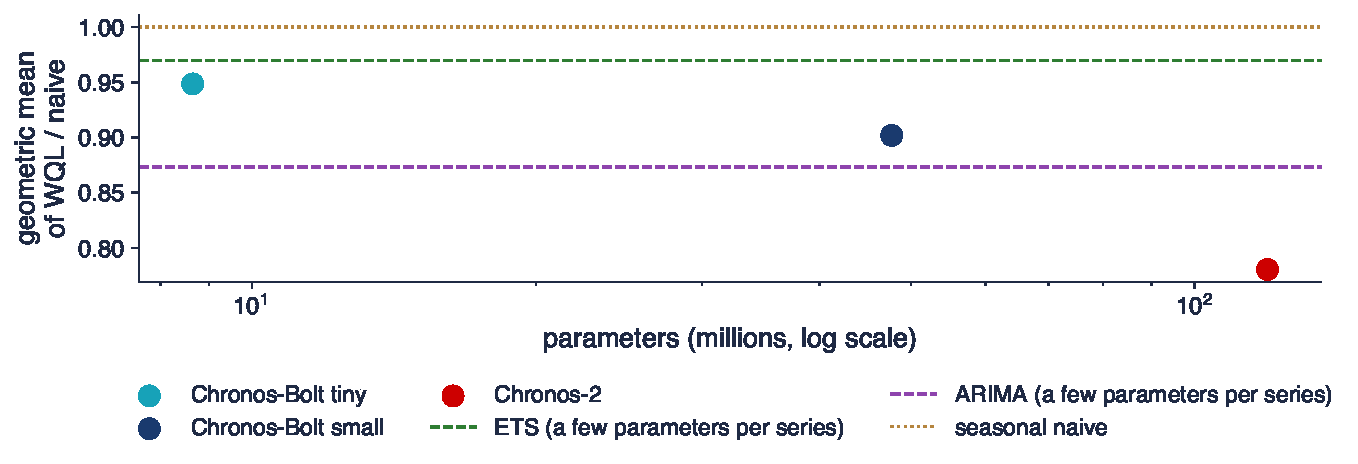
\includegraphics[width=0.97\textwidth,height=0.62\textheight,keepaspectratio]{tsa_ch11_size.pdf}
\end{center}
\vspace{-0.25cm}
\begin{itemize}
    \item Media geometrică, pe cele șapte serii, a raportului WQL față de prognoza sezonieră naivă, în funcție de numărul de parametri
\end{itemize}
\quantlet{TSA\_ch11\_context\_contamination}{\qlurl{TSA_ch11_context_contamination}}
\end{frame}

\begin{frame}{Interpretarea dimensiunii și a costului}
\itemsize{\small}
\begin{itemize}
    \item Parametri: Bolt tiny 9 milioane, Bolt small 48 de milioane, Chronos-2 119 milioane; ETS și ARIMA: cîțiva pe serie
    \item Precizia crește cu dimensiunea, dar ARIMA (0{,}87) se situează între modelul mic și cel mare
    \item Timpul pentru o prognoză a consumului pe procesorul unui laptop: Bolt small 19 ms, Chronos-2 43 ms, ARIMA 114 ms, ETS 411 ms
    \item Inferența zero-shot este ieftină; costul a fost plătit o singură dată, la pre-antrenare
\end{itemize}
\end{frame}

\begin{frame}{Benchmark-uri de referință}
\itemsize{\footnotesize}
\begin{itemize}
    \item \textbf{M3} (\refMH): 3003 serii; metodele sofisticate nu le-au bătut în medie pe cele simple
    \item \textbf{M4} (\refMSA): 100\,000 de serii; au cîștigat combinațiile și un hibrid de netezire exponențială și rețea neuronală
    \item \textbf{Arhiva Monash} (\refMonash): seturi publice de date cu orizonturi fixe și rezultate de referință
    \item \textbf{GIFT-Eval} (\refAksu): multe domenii și frecvențe, MASE și CRPS, un clasament public al foundation models
    \begin{itemize}
        \item separă datele de test de un corpus de pre-antrenare, pentru a limita contaminarea
    \end{itemize}
    \item Studii critice: modele liniare simple au bătut primele modele de prognoză cu Transformer (\refZeng); componentele LLM nu adaugă precizie (\refTan)
\end{itemize}
\end{frame}

\begin{frame}{Cînd ajută foundation models și cînd nu}
\itemsize{\footnotesize}
\begin{itemize}
    \item \textbf{Ajută}
    \begin{itemize}
        \item multe serii, puțin timp pentru fiecare; sezonalitate puternică și regulată; contexte lungi (consum, vînzări, trafic)
        \item un reper rapid și puternic înaintea unui model dedicat; ieșire probabilistă fără cost suplimentar
    \end{itemize}
    \item \textbf{Nu ajută}
    \begin{itemize}
        \item serii apropiate de un mers aleator (cursuri de schimb, randamente): nu este nimic de învățat din trecut
        \item serii scurte (cîteva zeci de trimestre), unde un ARIMA atent specificat este mai bun
        \item cînd contează factorii explicativi (temperatura, prețurile, politicile), iar aceștia nu sînt în context
        \item cînd modelul trebuie explicat parametru cu parametru sau se pune o întrebare cauzală
    \end{itemize}
    \item Comparați întotdeauna cu prognoza sezonieră naivă, ETS și ARIMA pe aceleași origini; testați diferențele cu Diebold--Mariano (\refDM)
\end{itemize}
\end{frame}

\begin{frame}{Recapitulare: evaluarea}
\itemsize{\small}
\begin{itemize}
    \item Chronos-2 este cel mai bun în medie, mai ales pentru consumul orar; ARIMA este aproape și cîștigă la PIB
    \item Pe seriile apropiate de un mers aleator, niciun model nu bate prognoza naivă
    \item Intervalele foundation models tind să fie prea înguste; contextul trebuie să acopere sezoanele
\end{itemize}
\end{frame}


%=============================================================================
\section{Scurgerea de informație și contaminarea}
%=============================================================================

\begin{frame}{Scurgerea de informație în propriul cod}
\itemsize{\footnotesize}
\begin{itemize}
    \item \textbf{Scurgerea de informație} (leakage): informația din perioada de test ajunge în prognoze (\refHew)
    \item Greșeli tipice
    \begin{itemize}
        \item scalarea sau standardizarea cu media întregului eșantion
        \item alegerea ordinelor ARIMA, a lungimii contextului sau a versiunii modelului după ce ați văzut erorile de test
        \item folosirea datelor revizuite (PIB) ca și cum ar fi fost cunoscute la origine
        \item împărțirea aleatoare a unei serii de timp în antrenare și test (\tsachlink{https://danpele.github.io/Time-Series-Analysis/RO/Cursuri/capitol9_invatare_automata_serii_timp.pdf}{Capitolul 9})
    \end{itemize}
    \item În acest capitol: fiecare context se termină la origine; ordinele ARIMA au fost fixate înaintea primei origini; Chronos scalează doar cu contextul
    \begin{itemize}
        \item problema rămasă: PIB-ul și producția de la Eurostat sînt ultima versiune revizuită, nu date în timp real
    \end{itemize}
\end{itemize}
\end{frame}

\begin{frame}{Contaminarea benchmark-urilor}
\itemsize{\footnotesize}
\begin{itemize}
    \item \textbf{Contaminarea}: seria de test (sau serii puternic corelate cu ea) a fost în corpusul de pre-antrenare
    \begin{itemize}
        \item scorul măsoară atunci memoria, nu prognoza: o distorsiune optimistă
    \end{itemize}
    \item Chronos raportează două benchmark-uri: în domeniu (seturi folosite la antrenare) și zero-shot (seturi nefolosite) (\refAnsari)
    \begin{itemize}
        \item serii publice precum M4 sau datele macro din SUA sînt probabil în multe corpusuri; FRED este public, la fel și Eurostat
    \end{itemize}
    \item Remedii
    \begin{itemize}
        \item testați doar pe date publicate după data lansării ponderilor
        \item benchmark-uri live: prognoze depuse înainte ca rezultatul să existe
        \item raportați corpusul de antrenare și data lansării fiecărui model folosit
    \end{itemize}
\end{itemize}
\end{frame}

\begin{frame}{O verificare a contaminării: înainte și după lansare}
\itemsize{\footnotesize}
\begin{center}
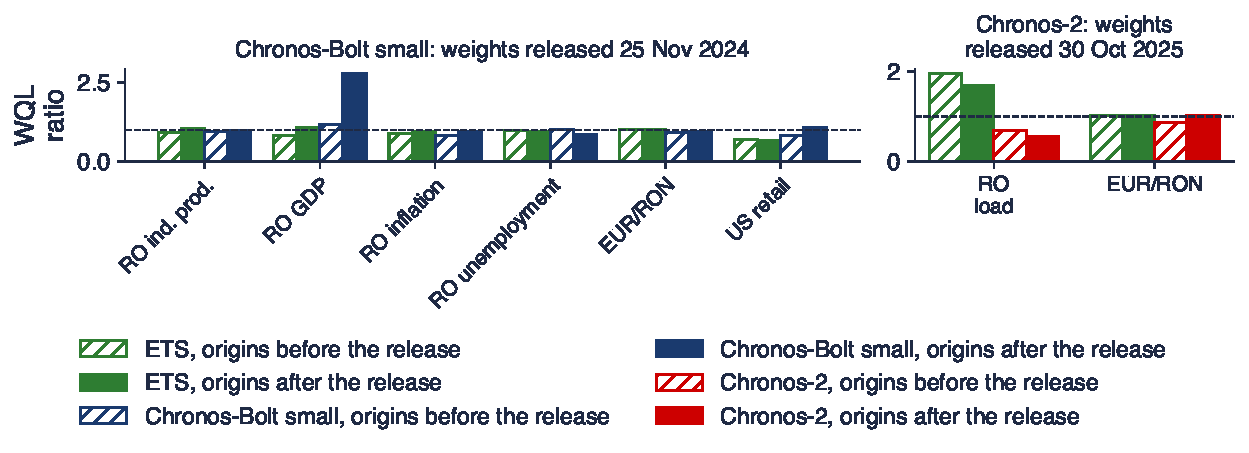
\includegraphics[width=0.97\textwidth,height=0.66\textheight,keepaspectratio]{tsa_ch11_prepost.pdf}
\end{center}
\vspace{-0.25cm}
\begin{itemize}
    \item Raportul WQL față de prognoza sezonieră naivă pentru originile dinainte (hașurat) și de după (plin) lansarea ponderilor; ETS pe aceleași origini, ca termen de comparație
\end{itemize}
\quantlet{TSA\_ch11\_context\_contamination}{\qlurl{TSA_ch11_context_contamination}}
\end{frame}

\begin{frame}{Interpretarea verificării contaminării}
\itemsize{\footnotesize}
\begin{itemize}
    \item Chronos-2 pe EUR/RON: 0{,}86 înainte de lansare (124 de origini), 1{,}02 după (10 origini): avantajul dispare
    \item Chronos-2 pe consum: 0{,}68 înainte, 0{,}54 după: cîștigul este real, și pe date pe care nu le-a putut vedea
    \item Chronos-Bolt small, vînzările din SUA: 0{,}82 înainte, 1{,}08 după, în timp ce ETS este stabil (0{,}69; 0{,}68)
    \item Atenție: 3--35 de origini după lansare sînt puține; și perioada de după diferă (2025--2026); o scădere este un semnal de alarmă, nu o dovadă
    \item Chronos-2 a fost lansat în octombrie 2025: rezultatele lui lunare de mai sus folosesc doar origini dinaintea acestei date
\end{itemize}
\end{frame}

\begin{frame}{Recapitulare: scurgerea de informație și contaminarea}
\itemsize{\small}
\begin{itemize}
    \item Scurgerea de informație este sub controlul dumneavoastră: folosiți doar datele disponibile la fiecare origine
    \item Contaminarea nu este: corpusul de pre-antrenare poate conține seria dumneavoastră
    \item Verificați rezultatele pe date publicate după lansarea modelului
\end{itemize}
\end{frame}


%=============================================================================
\section{Contribuția posibilă a AI}
%=============================================================================

\begin{frame}{Contribuția posibilă a AI}
\itemsize{\small}
\begin{itemize}
    \item \textbf{Cod}: o primă versiune a unui backtest cu origine mobilă, a pierderii pinball și a WQL, a unui fan chart
    \item \textbf{Lectură}: un rezumat al articolului unui model (arhitectura, corpusul, licența, data lansării)
    \item \textbf{Explorare}: rularea mai multor modele deschise pe multe serii românești de la Eurostat sau INS
    \item Exemplu de prompt
    \begin{itemize}
        \item \aiprompt{Write Python code that downloads Romanian monthly industrial production (Eurostat sts\_inpr\_m, not seasonally adjusted), forecasts 12 months ahead from monthly origins since 2016 with amazon/chronos-bolt-small (package chronos-forecasting, CPU), ETS and the seasonal naive, and reports MASE, the weighted quantile loss and the coverage of the 80\% interval.}
    \end{itemize}
\end{itemize}
\end{frame}

\begin{frame}{Verificări necesare}
\itemsize{\small}
\begin{itemize}
    \item Pachetul și numele modelelor: \texttt{BaseChronosPipeline}, \texttt{amazon/chronos-bolt-small}; o clasă sau un nume de model inventat eșuează imediat
    \item Contextul se termină la origine: nicio scalare, ordonare sau calibrare cu date de test
    \item Nivelurile cuantilelor: Chronos-Bolt dă doar 0,1--0,9; o „cuantilă de 1\%” obținută din el este o extrapolare
    \item Reperele: prognoza sezonieră naivă, ETS și ARIMA pe aceleași origini; scoruri relative la prognoza naivă
    \item Data lansării ponderilor comparată cu perioada de test; afirmațiile de tip „cel mai bun model” au nevoie de o sursă
    \item Fiecare articol citat: trebuie să existe; verificați numărul arXiv sau DOI-ul
\end{itemize}
\end{frame}


%=============================================================================
\section{Rezumat}
%=============================================================================

\begin{frame}{Idei de reținut}
\itemsize{\small}
\begin{itemize}
    \item Un foundation model este pre-antrenat o singură dată pe multe serii și prognozează serii noi zero-shot, doar din context
    \item Seriile devin intrări ale unui Transformer prin scalare, cuantizare (Chronos) sau patching (TimesFM, Moirai, Chronos-Bolt)
    \item Ieșirile sînt cuantile: evaluați-le cu pierderea pinball, CRPS sau WQL și verificați acoperirea
    \item Pe cele șapte serii: cîștiguri mari la consumul orar, niciunul la seriile apropiate de un mers aleator, pierderi la PIB-ul trimestrial scurt; ARIMA rămîne un reper puternic
    \item Contaminarea poate umfla scorurile publicate: testați pe date publicate după model
\end{itemize}
\end{frame}

\begin{frame}{Formule de reținut}
\itemsize{\small}
{\renewcommand{\arraystretch}{1.4}\begin{center}
\footnotesize
\begin{tabular}{ll}
\toprule
\textbf{Mărimea} & \textbf{Formula} \\
\midrule
Atenția & $\text{softmax}(QK^\top/\sqrt{d})\,V$ \\
Scalarea prin medie & $\tilde x_t = x_t/s$, \quad $s = \frac1C\sum_{t=1}^{C}|x_t|$ \\
Pierderea pinball & $L_\tau(y, q) = \max\{\tau(y - q),\ (\tau - 1)(y - q)\}$ \\
CRPS & $\int (F(z) - \mathbf{1}\{z \ge y\})^2\,dz = 2\int_0^1 L_\tau(y, F^{-1}(\tau))\,d\tau$ \\
WQL & $\frac{1}{K}\sum_{k=1}^{K} 2\sum_t L_{\tau_k}(y_t, \hat q_{\tau_k,t}) \big/ \sum_t |y_t|$ \\
MASE & $\frac1h\sum_j |y_{T+j} - \hat y_{T+j}| \Big/ \frac{1}{T-m}\sum_{t>m}|y_t - y_{t-m}|$ \\
Acoperirea & $\frac1n\sum \mathbf{1}\{\hat q_{0{,}1} \le y \le \hat q_{0{,}9}\}$, ținta 0,8 \\
\bottomrule
\end{tabular}
\end{center}
}
\end{frame}

\begin{frame}{Autoevaluare (1/2)}
\itemsize{\small}
\begin{itemize}
    \item \textbf{Întrebare}: care este diferența dintre prognoza zero-shot și fine-tuning?
    \begin{itemize}
        \item \textbf{Răspuns}: zero-shot păstrează fixe ponderile pre-antrenate și folosește doar contextul; fine-tuning-ul antrenează în continuare ponderile pe datele-țintă
    \end{itemize}
    \item \textbf{Întrebare}: un context este 10, 20, 30. Cît sînt $s$ și valorile scalate în Chronos?
    \begin{itemize}
        \item \textbf{Răspuns}: $s = 20$; valorile scalate 0,5; 1; 1,5
    \end{itemize}
    \item \textbf{Întrebare}: $\hat q_{0,9} = 5$ și $y = 6$. Cît este pierderea pinball?
    \begin{itemize}
        \item \textbf{Răspuns}: $0{,}9 \cdot (6 - 5) = 0{,}9$
    \end{itemize}
    \item \textbf{Întrebare}: cîte patch-uri de 16 dă un context de 512 valori?
    \begin{itemize}
        \item \textbf{Răspuns}: 32
    \end{itemize}
\end{itemize}
\end{frame}

\begin{frame}{Autoevaluare (2/2)}
\itemsize{\small}
\begin{itemize}
    \item \textbf{Întrebare}: un interval de 80\% acoperă 95\% din valorile observate. Este un rezultat bun?
    \begin{itemize}
        \item \textbf{Răspuns}: nu: intervalele sînt prea largi (lipsește precizia); CRPS penalizează acest lucru
    \end{itemize}
    \item \textbf{Întrebare}: de ce nu poate un foundation model să bată mersul aleator pe EUR/RON?
    \begin{itemize}
        \item \textbf{Răspuns}: variațiile cursului sînt aproape imprevizibile pe baza trecutului; niciun model nu poate extrage informație pe care contextul nu o conține
    \end{itemize}
    \item \textbf{Întrebare}: un model lansat în 2025 obține scoruri foarte bune pe date de test din 2018--2023. Ce verificați?
    \begin{itemize}
        \item \textbf{Răspuns}: dacă acele serii au fost în corpusul lui de pre-antrenare; repetați testul pe date publicate după lansare
    \end{itemize}
    \item \textbf{Idee de proiect}: comparați Chronos-Bolt, Chronos-2 și ARIMA pe toate seriile lunare ale României dintr-un set de date Eurostat, înainte și după datele de lansare
    \item Urmează: \tsachlink{https://danpele.github.io/Time-Series-Analysis/RO/Cursuri/capitol12_analiza_spectrala.pdf}{Capitolul 12}, analiza spectrală
\end{itemize}
\end{frame}


%=============================================================================
\section{Bibliografie}
%=============================================================================

\begin{frame}{Bibliografie (1/2)}
\itemsize{\tiny}
\begin{itemize}
    \item Aksu, T., Woo, G., Liu, J., Liu, X., et al.\ (2024). GIFT-Eval: A benchmark for general time series forecasting model evaluation. \href{https://arxiv.org/abs/2410.10393}{arXiv:2410.10393}
    \item Ansari, A. F., Stella, L., Turkmen, C., Zhang, X., et al.\ (2024). Chronos: Learning the language of time series. \textit{Transactions on Machine Learning Research}. \href{https://arxiv.org/abs/2403.07815}{arXiv:2403.07815}
    \item Ansari, A. F., Shchur, O., Küken, J., Auer, A., et al.\ (2025). Chronos-2: From univariate to universal forecasting. \href{https://arxiv.org/abs/2510.15821}{arXiv:2510.15821}
    \item Bommasani, R., Hudson, D. A., Adeli, E., Altman, R., et al.\ (2021). On the opportunities and risks of foundation models. \href{https://arxiv.org/abs/2108.07258}{arXiv:2108.07258}
    \item Das, A., Kong, W., Sen, R., \& Zhou, Y. (2024). A decoder-only foundation model for time-series forecasting. \textit{Proceedings of the 41st International Conference on Machine Learning (ICML)}. \href{https://arxiv.org/abs/2310.10688}{arXiv:2310.10688}
    \item Diebold, F. X., \& Mariano, R. S. (1995). Comparing predictive accuracy. \textit{Journal of Business \& Economic Statistics}, 13(3), 253--263. \href{https://doi.org/10.1080/07350015.1995.10524599}{doi:10.1080/07350015.1995.10524599}
    \item Garza, A., Challu, C., \& Mergenthaler-Canseco, M. (2023). TimeGPT-1. \href{https://arxiv.org/abs/2310.03589}{arXiv:2310.03589}
    \item Gneiting, T., \& Raftery, A. E. (2007). Strictly proper scoring rules, prediction, and estimation. \textit{Journal of the American Statistical Association}, 102(477), 359--378. \href{https://doi.org/10.1198/016214506000001437}{doi:10.1198/016214506000001437}
    \item Godahewa, R., Bergmeir, C., Webb, G. I., Hyndman, R. J., \& Montero-Manso, P. (2021). Monash time series forecasting archive. \textit{NeurIPS Track on Datasets and Benchmarks}. \href{https://arxiv.org/abs/2105.06643}{arXiv:2105.06643}
    \item Gruver, N., Finzi, M., Qiu, S., \& Wilson, A. G. (2023). Large language models are zero-shot time series forecasters. \textit{Advances in Neural Information Processing Systems}, 36. \href{https://arxiv.org/abs/2310.07820}{arXiv:2310.07820}
    \item Hewamalage, H., Ackermann, K., \& Bergmeir, C. (2023). Forecast evaluation for data scientists: Common pitfalls and best practices. \textit{Data Mining and Knowledge Discovery}, 37(2), 788--832. \href{https://doi.org/10.1007/s10618-022-00894-5}{doi:10.1007/s10618-022-00894-5}
    \item Huang, C., \& Petukhina, A. (2022). \textit{Applied Time Series Analysis and Forecasting with Python}. Springer. \href{https://doi.org/10.1007/978-3-031-13584-2}{doi:10.1007/978-3-031-13584-2}
    \item Hyndman, R. J., \& Athanasopoulos, G. (2021). \textit{Forecasting: Principles and Practice} (3rd ed.). OTexts. \href{https://otexts.com/fpp3/}{otexts.com/fpp3}
    \item Hyndman, R. J., \& Koehler, A. B. (2006). Another look at measures of forecast accuracy. \textit{International Journal of Forecasting}, 22(4), 679--688. \href{https://doi.org/10.1016/j.ijforecast.2006.03.001}{doi:10.1016/j.ijforecast.2006.03.001}
    \item Makridakis, S., \& Hibon, M. (2000). The M3-Competition: Results, conclusions and implications. \textit{International Journal of Forecasting}, 16(4), 451--476. \href{https://doi.org/10.1016/S0169-2070(00)00057-1}{doi:10.1016/S0169-2070(00)00057-1}
    \item Makridakis, S., Spiliotis, E., \& Assimakopoulos, V. (2020). The M4 Competition: 100,000 time series and 61 forecasting methods. \textit{International Journal of Forecasting}, 36(1), 54--74. \href{https://doi.org/10.1016/j.ijforecast.2019.04.014}{doi:10.1016/j.ijforecast.2019.04.014}
\end{itemize}
\end{frame}

\begin{frame}{Bibliografie (2/2)}
\itemsize{\tiny}
\begin{itemize}
    \item Matheson, J. E., \& Winkler, R. L. (1976). Scoring rules for continuous probability distributions. \textit{Management Science}, 22(10), 1087--1096. \href{https://doi.org/10.1287/mnsc.22.10.1087}{doi:10.1287/mnsc.22.10.1087}
    \item Nie, Y., Nguyen, N. H., Sinthong, P., \& Kalagnanam, J. (2023). A time series is worth 64 words: Long-term forecasting with Transformers. \textit{International Conference on Learning Representations (ICLR)}. \href{https://arxiv.org/abs/2211.14730}{arXiv:2211.14730}
    \item Rasul, K., Ashok, A., Williams, A. R., Ghonia, H., et al.\ (2023). Lag-Llama: Towards foundation models for probabilistic time series forecasting. \href{https://arxiv.org/abs/2310.08278}{arXiv:2310.08278}
    \item Salinas, D., Flunkert, V., Gasthaus, J., \& Januschowski, T. (2020). DeepAR: Probabilistic forecasting with autoregressive recurrent networks. \textit{International Journal of Forecasting}, 36(3), 1181--1191. \href{https://doi.org/10.1016/j.ijforecast.2019.07.001}{doi:10.1016/j.ijforecast.2019.07.001}
    \item Tan, M., Merrill, M. A., Gupta, V., Althoff, T., \& Hartvigsen, T. (2024). Are language models actually useful for time series forecasting? \textit{Advances in Neural Information Processing Systems}, 37. \href{https://arxiv.org/abs/2406.16964}{arXiv:2406.16964}
    \item Vaswani, A., Shazeer, N., Parmar, N., Uszkoreit, J., et al.\ (2017). Attention is all you need. \textit{Advances in Neural Information Processing Systems}, 30. \href{https://arxiv.org/abs/1706.03762}{arXiv:1706.03762}
    \item Woo, G., Liu, C., Kumar, A., Xiong, C., Savarese, S., \& Sahoo, D. (2024). Unified training of universal time series forecasting Transformers. \textit{Proceedings of the 41st International Conference on Machine Learning (ICML)}. \href{https://arxiv.org/abs/2402.02592}{arXiv:2402.02592}
    \item Zeng, A., Chen, M., Zhang, L., \& Xu, Q. (2023). Are Transformers effective for time series forecasting? \textit{Proceedings of the AAAI Conference on Artificial Intelligence}, 37(9), 11121--11128. \href{https://doi.org/10.1609/aaai.v37i9.26317}{doi:10.1609/aaai.v37i9.26317}
\end{itemize}
\end{frame}

\end{document}
